\chapter{CAT(0)-Räume} % (fold)
\label{cha:1}

\begin{definition}[Metrischer Raum]
\label{def:1.1}
	Sei $X$ eine Menge.\marginnote{21.10.15 \\ \ [1]}
	Eine Abbildung $d \colon X \times X \rightarrow \RR_{\geq 0}$ heißt \Index{Metrik}, wenn für alle $x,y,z \in X$ gilt:
	\begin{enumerate}[(i)]
		\item $d(x,y) = 0 \Leftrightarrow x=y$
		\item $d(x,y) = d(y,x)$
		\item $d(x,z) \leq d(x,y) + d(y,z)$
	\end{enumerate}
	Das Paar $(X,d)$ heißt dann \Index{metrischer Raum}.
\end{definition}

\begin{beispiel}
\label{bsp:1.2}
	\mbox{} \\[-1.4cm]
	\begin{enumerate}[(i)]
		\item Für $n \in \NN$ ist $\EE^n := (\RR^n,d_2)$ mit
		\begin{align*}
			d_2\colon \RR^n \times \RR^n &\longrightarrow \RR_{\geq 0} \\
			(x,y) &\longmapsto \sqrt{\sum_{i=1}^{n} (x_i-y_i)^2}.
		\end{align*}
		\item Sei $X$ eine Menge.
		Wir definieren:
		\begin{align*}
			d\colon X \times X &\longrightarrow \RR_{\geq 0} \\
			(x,y) &\longmapsto \begin{dcases}
				1, & x \neq y \\
				0, & x = y.
			\end{dcases}
		\end{align*}
		Dann ist $d$ eine Metrik und $(X,d)$ heißt ein \textbf{diskreter metrischer Raum}. \index{metrischer Raum!diskret}
	\end{enumerate}
\end{beispiel}

\begin{definition}[Geodätischer Raum]
\label{def:1.3}
	\mbox{} \\[-1.4cm]
	\begin{enumerate}[(i)]
		\item Sei $(X,d)$ ein metrischer Raum und $x,y \in X$.
		Eine \Index{Geodäte} von $x$ nach $y$ ist eine Abbildung $\gamma \colon [a,b] \rightarrow X$ mit $\gamma(a) = x, \gamma(b) = y$ und $d(\gamma(t),\gamma(t')) = \abs{t-t'}$ für alle $t,t' \in [a,b]$.
		Wir schreiben $\gamma\colon x \geo y$.
		\item Der Raum $(X,d)$ ist ein \Index{geodätischer Raum}, wenn für alle $x,y \in X$ eine Geodäte $x \geo y$ existiert.
		\item Ein geodätischer Raum heißt \textbf{eindeutig geodätisch}, wenn genau eine solche Geodäte existiert. \index{geodätischer Raum!eindeutig}
	\end{enumerate}
\end{definition}

Sofern nichts anderes gesagt wird, ist $[0,d(x,y)]$ der Definitionsbereich einer Geodäte $\alpha\colon x \geo y$.
\newpage
\begin{beispiel}
\label{bsp:1.4}
	\mbox{} \\[-1.4cm]
	\begin{enumerate}[(i)]
		\item Sei $(V, \Norm{\cdot})$ ein normierter reeller Vektorraum.
		Dann ist $(V,d_{\Norm{\cdot}})$ ein geodätischer Raum.
		Im Detail:
		Seien $u,v \in V$ paarweise verschieden und $L := \Norm{u-v} \neq 0$.
		Dann ist
		\begin{align*}
			\gamma\colon [0,L] &\longrightarrow V \\
			t &\longmapsto \enbrace*{1- \frac{t}{L}}\cdot u + \frac{t}{L} \cdot v
		\end{align*}
		eine Geodäte von $u$ nach $v$.
		\item $(\RR^2 \setminus \setzero, d_2)$ ist nicht geodätisch:
		Es existiert keine Geodäte $(-1,0) \geo (1,0)$.
		\item $(\RR^2,d_1)$ ist geodätisch, aber nicht eindeutig geodätisch:
		In der folgenden Abbildung sind zwei Geodäten von $(1,0) \geo (0,1)$ dargestellt.
		\begin{figure}[h]
		\centering
		\begin{tikzpicture}[scale=3,{>=Latex[]}]
			\draw[->] (-.2,0) -- (1.2,0);
			\draw[->] (0,-.2) -- (0,1.2);
			\draw (0,0) node[anchor=north east]{$0$};
			\draw (1,0.1) -- (1,-.1) node[below]{$1$};
			\draw (.1,1) -- (-.1,1) node[left]{$1$};
			
			\draw[->,very thick,color=red] (1,0) -- (0,1);
			\draw[->,very thick,color=blue] (1,.01) -- (.01,.01) -- (.01,1);
		\end{tikzpicture}
		\caption{Der metrische Raum $(\RR^2,d_1)$ ist nicht eindeutig geodätisch.}
		\end{figure}
	\end{enumerate}
\end{beispiel}

\begin{definition}[Geodätisches Dreieck]
\label{def:1.5}
	Ein \Index{geodätisches Dreieck} $\Delta = \Delta(x,y,z,\alpha,\beta,\gamma)$ in einem geodätischen Raum $(X,d)$ ist gegeben durch ein Tripel $(x,y,z) \in X^3$ und Geodäten $\alpha \colon x \geo y$, $\beta\colon y \geo z$, $\gamma \colon z \geo x$ -- den Seiten von $\Delta$.
\end{definition}

\begin{beispiel}
\label{bsp:1.6}
	\mbox{} \\[-1cm]
	\begin{figure}[h]
		\centering
		\begin{tikzpicture}[scale=2.5,>=Latex]
		\draw (-1,1) node[right]{$(\RR^2,d_1)$};
		\draw[->] (-1.1,0) -- (1.2,0);
		\draw[->] (0,-.3) -- (0,1.2);
		\draw (-1,.1) -- (-1,-.1) node[below]{$-1$};
		\draw (1,.1) -- (1,-.1) node[below]{$1$};
		\draw (-.1,1) -- (.1,1) node[right]{$1$};
		\draw[->,very thick, color=blue] (-1,0.02) -- (-0.02,0.02) -- (-0.02,1);
		\draw[->,very thick, color=red] (0.02,1) -- (0.02,0.02) -- (1,0.02);
		\draw[->,very thick, color=SeaGreen4] (1,-0.02) -- (-1,-0.02);
		\end{tikzpicture} \hspace{2cm}
		\begin{tikzpicture}[scale=2.5,>=Latex]
			\draw (-1,1) node[right]{$(\RR^2,d_1)$};
			\draw[->] (-1.1,0) -- (1.2,0);
			\draw[->] (0,-.3) -- (0,1.2);
			\draw (-1,.1) -- (-1,-.1) node[below]{$-1$};
			\draw (1,.1) -- (1,-.1) node[below]{$1$};
			\draw (-.1,1) -- (.1,1) node[right]{$1$};
			
		\draw[->,very thick, color=blue] (-1,0) -- (0,1);
		\draw[->,very thick, color=red] (0,1) -- (1,0);
		\draw[->,very thick, color=SeaGreen4] (1,0.02) -- (-1,0.02);
		\end{tikzpicture}
		\caption{Geodätische Dreiecke sind im Allgemeinen durch ihre Ecken nicht eindeutig bestimmt.}
	\end{figure}
\end{beispiel}

Die Dreiecksungleichung garantiert, dass es Punkte $\ol{x},\ol{y},\ol{z} \in \EE^2$ gibt mit $d(x,y) = d_2(\ol{x},\ol{y})$, $d(y,z) = d_2(\ol{y},\ol{z})$, $d(z,x) = d_2(\ol{z},\ol{x})$ und Geodäten
\[
	\ol{\alpha}(t) = \ol{x} + t \cdot \frac{\ol{y}-\ol{x}}{d_2(\ol{y},\ol{x})}, \qquad \ol{\beta}(t) = \ol{y} + t \cdot \frac{\ol{z}-\ol{y}}{d_2(\ol{z},\ol{y})}, \qquad
	\ol{\gamma}(t) = \ol{z} + t \cdot \frac{\ol{x}-\ol{z}}{d_2(\ol{x},\ol{z})}.
\]
$\ol{\Delta} = \ol{\Delta}(\ol{x},\ol{y},\ol{z},\ol{\alpha},\ol{\beta},\ol{\gamma})$ heißt \Index{Vergleichsdreieck} zu $\Delta(x,y,z,\alpha,\beta,\gamma)$.
Ist $v = \gamma(s)$ für ein $s$, so heißt $\ol{v} = \ol{\gamma}(s)$ \Index{Vergleichspunkt} von $v$.

\begin{definition}[$\CAT$-Raum]
\label{def:1.7}
	\mbox{} \\[-1.4cm]
	\begin{enumerate}[(i)]
		\item Ein Dreieck $\Delta$ in $(X,d)$ hat die \textbf{CAT(0)-Eigenschaft}, wenn für alle $n,m$ auf den Seiten von $\Delta$ und ihre Vergleichspunkte $\ol{n},\ol{m}$ auf den Seiten von $\ol{\Delta}$ gilt: \index{CAT(0)-Raum@$\CAT$-Raum}
		\[
			d(n,m) \leq d_2(\ol{n},\ol{m})
		\]
		\item Ein metrischer Raum $(X,d)$ ist ein \textbf{CAT(0)-Raum}, wenn $(X,d)$ geodätisch ist und alle seine Dreiecke die $\CAT$-Eigenschaft erfüllen.
		\item Ein metrischer Raum $(X,d)$ heißt \textbf{lokal CAT(0)}, wenn für alle $x \in X$ ein $r_x > 0$ existiert, sodass
		\[
			B_{r_x}(x) = \{y \in X : d(y,x) < r_x\}
		\]
		mit der induzierten Metrik ein $\CAT$-Raum ist. \index{CAT(0)-Raum@$\CAT$-Raum!lokal}
	\end{enumerate}
\end{definition}

\begin{figure}[h]
	\centering
	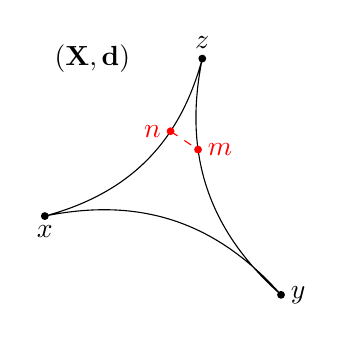
\begin{tikzpicture}[scale=1]
	\draw (0,1) node[fill,circle,inner sep=1pt]{}
	to [bend left] (3,0) node[fill,circle,inner sep=1pt]{} 
	to [bend left] coordinate[pos=.66] (M) (2,3) node[fill,circle,inner sep=1pt]{}
	to [bend left] coordinate[pos=.33] (N) cycle;
	\draw (0,1) node[below]{$x$};
	\draw (3,0) node[right]{$y$};
	\draw (2,3) node[above]{$z$};
	\draw (N) node[fill,circle,inner sep=1pt,color=red]{};
	\draw (N) node[left,color=red]{$n$};
	\draw (M) node[fill,circle,inner sep=1pt,color=red]{};
	\draw (M) node[right,color=red]{$m$};
	\draw[color=red, dashed] (N) -- (M);
	\draw (0,3) node[right]{$\mathbf{(X,d)}$};
	\end{tikzpicture} \hspace{2cm}
	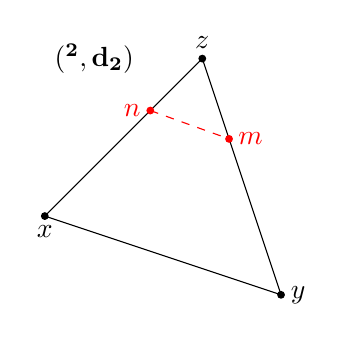
\begin{tikzpicture}[scale=1]
	\draw (0,1) node[fill,circle,inner sep=1pt]{}
	to (3,0) node[fill,circle,inner sep=1pt]{} 
	to coordinate[pos=.66] (M) (2,3) node[fill,circle,inner sep=1pt]{}
	to coordinate[pos=.33] (N) cycle;
	\draw (0,1) node[below]{$\ol{x}$};
	\draw (3,0) node[right]{$\ol{y}$};
	\draw (2,3) node[above]{$\ol{z}$};
	\draw (N) node[fill,circle,inner sep=1pt,color=red]{};
	\draw (N) node[left,color=red]{$\ol{n}$};
	\draw (M) node[fill,circle,inner sep=1pt,color=red]{};
	\draw (M) node[right,color=red,xshift=-.2]{$\ol{m}$};
	\draw[color=red, dashed] (N) -- (M);
	\draw (0,3) node[right]{$\mathbf{(\RR^2,d_2)}$};
	\end{tikzpicture}	
	\caption{Anschaulich gesprochen sind Dreiecke in $\CAT$-Räumen \enquote{mindestens so dünn} wie ihre Vergleichsdreiecke im euklidischen Raum.}
\end{figure}

\begin{bemerkung}
\label{bem:1.8}
	\mbox{} \\[-1.4cm]
	\begin{enumerate}[(i)]
		\item Lokal $\CAT$-Räume heißen auch nichtpositiv gekrümmte oder Alexandrov-Räume.
		\item $\CAT$ steht für \textsc{Cartan-Alexandrov-Topogonov} und Krümmung $\leq 0$.
	\end{enumerate}
\end{bemerkung}
\newpage
\begin{beispiel}
\label{bsp:1.9}
	\mbox{} \\[-1.4cm]
	\begin{enumerate}[(i)]
		\item Der euklidische Raum $\EE^n$ ist $\CAT$.
		\item $(\RR^2,d_1)$ ist nicht $\CAT$: In der folgenden Abbildung~\ref{abb:1.4} ist $d_1(n,m) = 2$, aber $d_2(\ol{n},\ol{m}) = \sqrt{3}$.
		\begin{figure}[h]
			\centering
			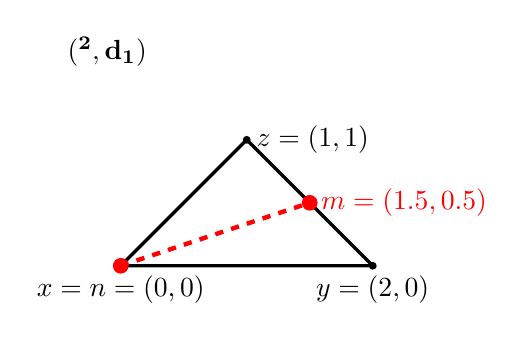
\begin{tikzpicture}[scale=1.6]	
			\draw (-1,0) node[below]{$x = n = (0,0)$};
			\draw (1,0) node[below]{$y = (2,0)$};
			\draw (0,1) node[right]{$z = (1,1)$};
			
			\draw[very thick] (-1,0) node[fill,circle,inner sep=2pt,color=red]{} -- (1,0) node[fill,circle,inner sep=1pt]{} -- coordinate[pos=.5] (M) (0,1) node[fill,circle,inner sep=1pt]{} -- cycle;
			
			\draw (M) node[fill,circle,inner sep=2pt,color=red]{};
			\draw (M) node[right,color=red,xshift=.6]{$m = (1.5,0.5)$};
			\draw[color=red,dashed,ultra thick] (-1,0) -- (M);
			\draw (-1.5,1.7) node[right]{$\mathbf{(\RR^2,d_1)}$};
			\end{tikzpicture} \hspace{1.5cm}
			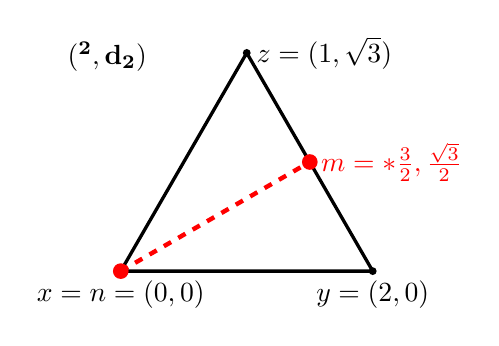
\begin{tikzpicture}[scale=1.6]	
			\draw[very thick] (0,0) node[fill,circle,inner sep=2pt,color=red]{} -- (2,0) node[fill,circle,inner sep=1pt]{} -- coordinate[pos=.5] (M) (1,1.732051) node[fill,circle,inner sep=1pt]{} -- cycle;
			
			\draw (0,0) node[below]{$\ol{x} = \ol{n} =(0,0)$};
			\draw (2,0) node[below]{$\ol{y} = (2,0)$};
			\draw (1,1.732051) node[right]{$\ol{z} = (1,\sqrt{3})$};
			
			\draw (M) node[fill,circle,inner sep=2pt,color=red]{};
			\draw (M) node[right,color=red,xshift=.6]{$\ol{m} = \enbrace*{\frac{3}{2},\frac{\sqrt{3}}{2}}$};
			\draw[color=red,dashed,ultra thick] (0,0) -- (M);
			\draw (-0.5,1.7) node[right]{$\mathbf{(\RR^2,d_2)}$};	
			\end{tikzpicture}
			\caption{Der Raum $(\RR^2,d_1)$ ist nicht $\CAT$.}
			\label{abb:1.4}
		\end{figure}
		\item Hilberträume sind $\CAT$.
		\item Komplemente von Polygonen im $\RR^2$ sind lokal $\CAT$, aber nicht $\CAT$.	
	\end{enumerate}
\end{beispiel}

\begin{beobachtung}
\label{beob:1.10}
	Sei $(X,d)$ ein $\CAT$-Raum.
	Dann ist $X$ eindeutig geodätisch.
\end{beobachtung}

\begin{beweis}
	Seien $\gamma\colon x \geo y$ und $\gamma'\colon x \geo y$ zwei Geodäten von $x$ nach $y$.
	Seien $p$ und $p'$ zwei Punkte auf $\gamma$ und $\gamma'$ mit $d(x,p) = d(x,p')$.
	Das Vergleichsdreieck $\ol{\Delta}$ zum Dreieck
	\[
		\Delta = \Delta\enbrace*{x,p,y,\gamma \big|_{[0,d(x,p)]}, \gamma \big|_{[d(x,p),d(x,y)]},\gamma'}
	\]
	ist degeneriert:
	\begin{figure}[h]
		\centering
		\begin{tikzpicture}[scale=1.5,>=Latex]
			\draw (0,0) node[fill,circle,inner sep=1.5pt,color=black]{};
			\draw (3,0) node[fill,circle,inner sep=1.5pt,color=black]{};
			\draw [->,very thick,color=red] (0,0) to [bend left] coordinate[pos=0.3] (P) (3,0);
			\draw [->,very thick,color=blue] (0,0) to [bend right] coordinate[pos=0.3] (Q) (3,0);
			
			\draw (0,0) node[left]{$x$};
			\draw (3,0) node[right]{$y$};
			
			\draw (P) node[fill,circle,inner sep=1.5pt,color=black]{};
			\draw (Q) node[fill,circle,inner sep=1.5pt,color=black]{};
			\draw (P) node[above]{$p$};
			\draw (Q) node[below]{$p'$};
			
			\draw[color=red] (1.5,.5) node[above]{$\gamma$};
			\draw[color=blue] (1.5,-.5) node[below]{$\gamma'$};
		\end{tikzpicture} \hspace{2cm}
		\begin{tikzpicture}[scale=1.5,>=Latex]
		\draw (0,0) node[fill,circle,inner sep=1.5pt,color=black]{};
		\draw (3,0) node[fill,circle,inner sep=1.5pt,color=black]{};
		\draw [->,very thick,color=red] (0,0.01) to coordinate[pos=0.3] (P) (3,0.01);
		\draw [->,very thick,color=blue] (0,-0.01) to  coordinate[pos=0.3] (Q) (3,-0.01);
		
		\draw (0,0) node[left]{$\ol{x}$};
		\draw (3,0) node[right]{$\ol{y}$};
		
		\draw (P) node[fill,circle,inner sep=1.5pt,color=black]{};
		\draw (Q) node[fill,circle,inner sep=1.5pt,color=black]{};
		\draw (P) node[above]{$\ol{p}$};
		\draw (Q) node[below]{$\ol{p'}$};
		
		\draw[color=red] (1.5,.1) node[above]{$\ol{\gamma}$};
		\draw[color=blue] (1.5,-.1) node[below]{$\ol{\gamma'}$};
		\end{tikzpicture}
	\end{figure}
	
	Wegen der $\CAT$-Eigenschaft gilt $d(p,p') \leq d(\ol{p},\ol{p'}) = 0$, also folgt $d(p,p')=0$ und $p = p'$.
\end{beweis}

\begin{definition}[Konvexe Menge]
\label{def:1.11}
	Sei $X$ ein $\CAT$-Raum. Eine nichtleere Teilmenge $C \subseteq X$ heißt \Index{konvex}, wenn zu allen $p,q \in C$ die Geodäte $\gamma \colon p \geo q$ in $C$ liegt.
\end{definition}

Offensichtlich ist $C$ wieder ein $\CAT$-Raum und Durchschnitte konvexer Mengen sind wieder konvex.

\begin{theorem}[{\cite[\hspace{0cm}1A.6]{BridsonHaefliger}}]
\label{th:1.12}
	Sei $\mathcal{M}$ eine einfach zusammenhängende Riemannsche Mannigfaltigkeit nichtpositiver Krümmung. \marginnote{23.10.15 \\ \ [2]}
	Dann ist $\mathcal{M}$ $\CAT$.	
\end{theorem}

\begin{satz}
\label{satz:1.13}
	Sei $(V,\Norm{\cdot})$ ein reeller normierter Vektorraum.
	Dann ist $(V,\Norm{\cdot})$ genau dann ein $\CAT$-Raum, wenn $(V,\Norm{\cdot})$ ein Prähilbertraum ist, das heißt es existiert eine symmetrische positiv definite Bilinearform $\sprod{\cdot,\cdot}\colon V \times V \rightarrow \RR$ mit $\Norm{v} = \sqrt{\sprod{v,v}}$ für $v \in V$.
\end{satz}

Für den Beweis brauchen wir eine metrische Charakterisierung von Prähilberträumen:

\vspace*{.5cm}

\begin{minipage}{0.6\textwidth}
	\begin{proposition}[\textsc{von Neumann}, 1935]
		\label{prop:1.14}
		Ein reeller normierter Vektorraum $(V,\Norm{\cdot})$ ist ein Prähilbertraum genau dann, wenn für alle $v,w \in V$ die \Index{Parallelogrammgleichung} gilt:
		\begin{align}
		\Norm{v-w}^2 + \Norm{v+w}^2 = 2 \cdot (\Norm{v}^2 + \Norm{w}^2) \tag{PG} \label{eq:PG}
		\end{align}
	\end{proposition}
\end{minipage}
~
\begin{minipage}{0.35\textwidth}
		\begin{tikzpicture}[scale=1,>=Latex]
		\draw (0,0) node[fill,circle,inner sep=1.5pt]{};
		\draw (1,2) node[fill,circle,inner sep=1.5pt]{};
		\draw (4,1) node[fill,circle,inner sep=1.5pt]{};
		\draw (5,3) node[fill,circle,inner sep=1.5pt]{};
		
		\draw (0,0) node[left]{$0$};
		\draw (1,2) node[left]{$v$};
		\draw (4,1) node[right]{$w$};
		\draw (5,3) node[right]{$v+w$};
		\draw (3.3,1.33) node[rotate=-20]{$\Norm{v-w}$};
		
		\draw [->,thick] (0,0) -- (1,2);
		\draw [->,thick] (0,0) -- (5,3);
		\draw [->,thick] (0,0) -- (4,1);
		\draw [thick,dashed] (1,2) -- (5,3) -- (4,1) -- cycle;
		\end{tikzpicture}
\end{minipage}

\begin{beweis}
	\mbox{} \\[-.85cm]
	\begin{description}
		\item[\bewhin] Seien $u,v \in V$.
		\begin{align*}
			&\Norm{u-v}^2 + \Norm{u+v}^2 \\
			= \  &\sprod{u-v,u-v} + \sprod{u+v,u+v} \\
			= \ &\sprod{u,u} - \sprod{u,v} - \sprod{v,u} + \sprod{v,v} + \sprod{u,u} + \sprod{u,v} + \sprod{v,u} + \sprod{v,v} \\
			= \ &2 \cdot (\sprod{v,v}^2 + \sprod{u,u}^2)
		\end{align*}
		\item[\bewrueck] Definiere:
		\begin{align*}
			b\colon V \times V &\longrightarrow \RR \\
			(u,v) &\longmapsto \frac{1}{4} ( \Norm{u+v}^2 - \Norm{u-v}^2).
		\end{align*} 
		Wir zeigen, dass $b$ ein Skalarprodukt ist: 
		\begin{itemize}
			\item Offensichtlich ist $b$ symmetrisch.
			\item $b$ ist positiv definit, denn für $v \in V$ gilt:
			\begin{align*}
				b(v,v) &= \frac{1}{4} (2\cdot \Norm{v})^2 = \Norm{v}^2 \geq 0 \\
				b(v,v) &= 0 \Leftrightarrow v = 0
			\end{align*}
			\item Sei nun $w \in V$ beliebig. Zu zeigen ist, dass $b(\cdot,w) \colon V \rightarrow \RR$ linear ist. Seien also $u,v \in V$ beliebig, dann gilt:
			\begin{align}
				&b(u+v,w) + b(u-v,w) \\
				\stack{\text{Def}}{=} &\frac{1}{4} (\Norm{\textcolor{blue}{u}+v+\textcolor{blue}{w}}^2 - \Norm{\textcolor{red}{u}+v\textcolor{red}{-w}}^2 + \Norm{\textcolor{blue}{u}-v+\textcolor{blue}{w}}^2 - \Norm{\textcolor{red}{u}-v\textcolor{red}{-w}}^2) \\
				\stack{\eqref{eq:PG}}{=} &\frac{1}{4} (2 \cdot \Norm{u+w}^2 + 2 \cdot \Norm{v}^2 - 2 \cdot \Norm{u-w}^2 - 2\cdot \Norm{v}^2) \\
				\stack{}{=} &\frac{1}{2} (\Norm{u+w}^2 - \Norm{u-w}^2) \\
				\stack{\text{Def}}{=} &2 \cdot b(u,w) \label{eq:1.14.1}
			\end{align}
			Analog erhalten wir
			\begin{equation}
				b(u+v,w) - b(u-v,w) = 2 \cdot b(v,w). \label{eq:1.14.2}
			\end{equation}
			Addition von \eqref{eq:1.14.1} und \eqref{eq:1.14.2} liefert:
			\[ b(u+v,w) = b(u,w) + b(v,w) \]
			Bleibt zu zeigen: Für alle $r \in \RR$ gilt $b(rv,w) = r\cdot b(v,w)$.
			\begin{description}
				\item[1. Fall:] $r=-1$.
				Mit $u = 0$ folgt aus \eqref{eq:1.14.1}:
				\[
					b(v,w) + b(-v,w) = 2 \cdot b(0,w) = 2 \cdot \frac{1}{4} (\Norm{w}^2 - \Norm{-w}^2) = 0
				\]
				und somit $b(-v,w) = -b(v,w)$.
				\item[2. Fall:] $r = n \in \NN$.
				Für $n = 2$ folgt mit $u = v$ aus \eqref{eq:1.14.1}
				\[
					b(2v,w) + \Underbrace{b(0,w)}{=0} = 2 \cdot b(v,w)
				\]
				und weiter induktiv
				\begin{align*}
					b(nv,w) &= b((n-1)v + v,w) = b((n-1)v,w) + b(v,w) \\
					&= (n-1) b(v,w) + b(v,w) = n\cdot b(v,w).
				\end{align*}
				\item[3. Fall:] $r = \frac{1}{n}$ mit $n \in \NN, n \geq 1$.
				Es gilt $\frac{1}{n} \cdot b(nv,w) = b(v,w)$ und damit
				\[
					b\enbrace*{\frac{1}{n} v,w} = \frac{1}{n} \cdot b(n \cdot \frac{1}{n}v,w) = \frac{1}{n} b(v,w)
				\] 
			\end{description}
			Aus allen drei Fällen folgt nun $b(qv,w) = q\cdot b(v,w)$ für alle $q \in \QQ$. Da $\QQ \subseteq \RR$ eine dichte Teilmenge und $b(\cdot,w)$ stetig ist, folgt $b(rv,w) = r \cdot b(v,w)$ für alle $r \in \RR$. \qedhere
		\end{itemize}
	\end{description}
\end{beweis}

\begin{beweis}[Satz~\ref{satz:1.13}]
	\mbox{} \\[-.85cm]
	\begin{description}
		\item[\bewrueck] Sei $\Delta \subseteq (V,\Norm{\cdot}) = \HH$ ein geodätisches Dreieck.
		Dann ist die lineare Hülle $\sprod{\Delta}$ isometrisch isomorph zum $\EE^2$, bzw. zum $\EE^1$ oder zu $\setzero$, falls $\Delta$ degeneriert ist.
		\item[\bewhin] Sei $u,v \in V$ beliebig.
		Zeige, dass für $v,w$ das Parallelogrammgesetz gilt:
		Wir betrachten das Dreieck $\Delta(0,u,v)$ und das Vergleichsdreieck $\ol{\Delta}(0,\ol{u},\ol{v})$.
		Es gilt:
		\begin{align}
			d\enbrace*{\frac{u+v}{2},0} &\makebox[1cm][c]{$\stackrel{\CAT}{\leq}$} d_2\enbrace*{\frac{\ol{u}+\ol{v}}{2},0} \\
			\Rightarrow  d(u+v,0) &\makebox[1cm][c]{$\leq$} d_2(\ol{u}+\ol{v},0) \\
			\Rightarrow \Norm{u+v}^2 \leq \Norm{\ol{u}+\ol{v}}_2^2 &\makebox[1cm][c]{$\stackrel{\eqref{eq:PG}}{=}$} 2 \cdot \Norm{\ol{u}}_2^2 + 2 \cdot \Norm{\ol{v}}_2^2 - \Norm{\ol{u}-\ol{v}}_2^2 \\
			&\makebox[1cm][c]{$\stackrel{\CAT}{=}$} 2 \cdot \Norm{u}^2 + 2 \cdot \Norm{v}^2 - \Norm{u-v}^2 \label{eq:1.13.1}
		\end{align}
		Betrachte das Dreieck $\Delta(0-v,u)$ und das Vergleichsdreieck $\ol{\Delta}(0-\ol{v},\ol{u})$.
		Wir erhalten genauso wie oben die Ungleichung
		\begin{equation}
			\Norm{u-v}^2 \leq 2 \cdot \Norm{u}^2 + 2 \cdot \Norm{v}^2 - \Norm{u+v}^2. \label{eq:1.13.2}
		\end{equation}
		Insgesamt haben wir also:
		\[
			\Norm{u+v}^2 \stackrel{\eqref{eq:1.13.1}}{\leq} 2 \cdot \Norm{u}^2 + 2\cdot \Norm{v}^2 - \Norm{u-v}^2 \stackrel{\eqref{eq:1.13.2}}{\leq} \Norm{u+v}^2 \qedhere
		\]
	\end{description}
\end{beweis}

\vspace*{.5cm}

\begin{minipage}{0.6\textwidth}
\begin{erinnerung}[Orthogonale Projektion]
\label{erin:1.15}
	Gegeben sei ein reeller Hilbertraum $\EE^d$ und $U \subseteq \EE^d$ ein Unterraum.
	Sei weiter $v_1,\dots,v_n \in U$ eine Orthonormalbasis von $U$.
	Dann ist \index{orthogonale Projektion}
	\begin{align*}
		\pi_U \colon V &\longrightarrow U \\
		v &\longmapsto \sum_{i=0}^{n} \sprod{v,v_i} \cdot v_i
	\end{align*}
	eine lineare Abbildung und es gilt
	\[
		d(v,\pi_U(v)) = \inf_{u\in U} d(v,u) =: d(v,U)
	\]
	und $v- \pi_U(v) \perp U$.
\end{erinnerung}
\end{minipage} \hspace{.5cm}
\begin{minipage}{0.35\textwidth}
	\begin{tikzpicture}[scale=2,>=Latex]
		\draw [->] (-.2,0) -- (2,0);
		\draw [->] (0,-.2) -- (0,2);
		
		\draw [thick] (-.2,-.1) -- (1.5,.75) node[anchor=south west]{$U$};
		\draw [thick,dashed] (.5,1.5) node[right]{$v$} -- (1,.5) node[anchor=north west,color=red]{$\pi_U(v)$};
		\draw (.5,1.5) node[fill,circle,inner sep=1.5pt]{};
		\draw (1,.5) node[fill,circle,inner sep=1.5pt,color=red]{};
	\end{tikzpicture}
\end{minipage}

\begin{satz}[Projektion auf konvexe Teilmengen]
\label{satz:1.16}
	Sei $X$ ein $\CAT$-Raum und $C \subseteq X$ konvex und vollständig mit der induzierten Metrik.
	Dann gilt:
	\begin{enumerate}[(i)]
		\item Für alle $x \in X$ existiert genau ein $\pi_C(x) \in C$ mit
		\[
			d(x,\pi_C(x)) = \inf_{p \in C} d(x,p) =: d(x,C).
		\]
		Die Abbildung $\pi_C \colon X \rightarrow C$ heißt die \textbf{(orthogonale) Projektion} auf $C$. \index{orthogonale Projektion}
		\newpage
		\item Ist $y \in [x, \pi_C(x)] = \im(\gamma \colon x \geo \pi_C(x))$, so ist $\pi_C(y) = \pi_C(x)$.
		\begin{figure}[h]
			\centering
		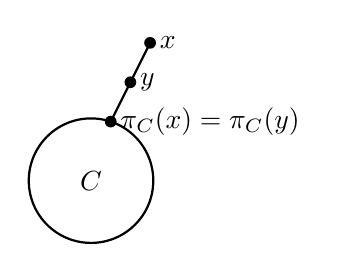
\begin{tikzpicture}[scale=.5]
			\draw [thick] (0.5,0.5) circle (1.58113883);
			\draw [thick] (1,2) node[fill,circle,inner sep=1.5pt]{} -- (1.5,3) node[fill,circle,inner sep=1.5pt]{} -- (2,4) node[fill,circle,inner sep=1.5pt]{};
			
			\draw (0.5,0.5) node{$C$};
			\draw (1,2) node[right]{$\pi_C(x) = \pi_C(y)$};
			\draw (1.5,3) node[right]{$y$};
			\draw (2,4) node[right]{$x$};
		\end{tikzpicture}
		\end{figure}
		\item Für alle $x,y \in X$ gilt
		\[
			d(\pi_C(x),\pi_C(y)) \leq d(x,y),
		\]
		das heißt $\pi_C$ ist $1$-Lipschitz. \index{Lipschitz}
	\end{enumerate}
\end{satz}

\begin{beweis}
	\mbox{}\\[-.85cm]
	\begin{enumerate}[(i)]
		\item Sei $(y_n)_{n \in \NN} \subseteq C$ eine Folge mit $d(x,y_n) \rightarrow d(x,C) =: D$.
		Ziel ist es zu zeigen, dass $(y_n)_n$ eine Cauchy-Folge ist.
		Da $C$ vollständig ist, ist die Folge $(y_n)_n$ konvergent in $C$ und wir können $\pi_C(x) := \lim\limits_{n \rightarrow \infty} y_n$ definieren.
		
		Zur Eindeutigkeit von $\pi_C(x)$: Angenommen, es existiert ein $\pi_C(x') \in C$ mit $\pi_C(x)' \neq \pi_C(x)$ und $d(x,\pi_C(x)') = d(x,C)$. Betrachte die Folge
		\[
			q_n := \begin{dcases}
				\pi_C(x), & n \text{ gerade} \\
				\pi_C(x)', & n \text{ ungerade}.
			\end{dcases}
		\]
		Dann ist $d(x,q_n) \rightarrow d(x,C)$, aber $(q_n)_n$ ist keine Cauchy-Folge. Widerspruch.
		
		Zur Existenz: Betrachte folgendes Dreieck und Vergleichsdreieck ergänzt zu einem Parallelogramm:
		
		\begin{figure}[h]
			\centering
			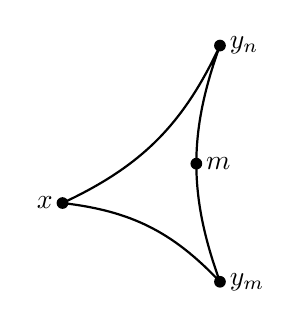
\begin{tikzpicture}[scale=1]
				\draw (0,0) node[fill,circle,inner sep=1.5pt]{};
				\draw (2,-1) node[fill,circle,inner sep=1.5pt]{};
				\draw (2,2) node[fill,circle,inner sep=1.5pt]{};
				
				\draw[thick] (0,0) to [bend angle=20, bend left] (2,-1) to [bend angle=20, bend left] coordinate[pos=.5] (M) (2,2) to [bend angle=20, bend left] (0,0);
				
				\draw (0,0) node[left]{$x$};
				\draw (2,-1) node[right]{$y_m$};
				\draw (2,2) node[right]{$y_n$};
				\draw (M) node[fill,circle,inner sep=1.5pt]{};
				\draw (M) node[right]{$m$};
			\end{tikzpicture} \hspace{1cm}
			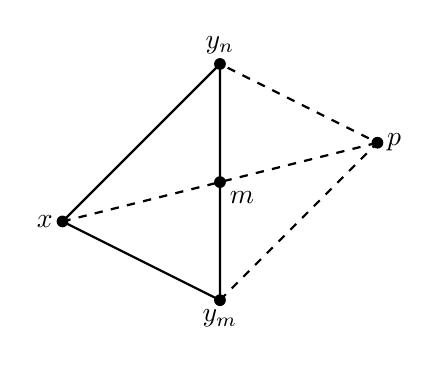
\begin{tikzpicture}[scale=1]
				\draw (0,0) node[fill,circle,inner sep=1.5pt]{};
				\draw (2,-1) node[fill,circle,inner sep=1.5pt]{};
				\draw (2,2) node[fill,circle,inner sep=1.5pt]{};
				\draw (4,1) node[fill,circle,inner sep=1.5pt]{};
				
				\draw[thick] (0,0) to (2,-1) to coordinate[pos=.5] (M) (2,2) to (0,0);
				\draw[thick,dashed] (2,-1) -- (4,1) -- (2,2);
				\draw[thick,dashed] (0,0) -- (4,1);
				
				\draw (0,0) node[left]{$\ol{x}$};
				\draw (2,-1) node[below]{$\ol{y_m}$};
				\draw (2,2) node[above]{$\ol{y_n}$};
				\draw (4,1) node[right]{$\ol{p}$};
				\draw (M) node[fill,circle,inner sep=1.5pt]{};
				\draw (M) node[anchor=north west]{$\ol{m}$};
			\end{tikzpicture}
			\caption{Zu einem Parallelogramm ergänztes Vergleichsdreieck.}
			\label{abb:erg_parallel}
		\end{figure}
		
		Es ist $d(y_n,m) = d(y_m,m) = \frac{1}{2} d(y_n,y_m)$.
		Die Parallelogrammgleichung in $\EE^2$ besagt:
		\[
			d_2(\ol{x},\ol{p})^2 + d_2(\ol{y_n},\ol{y_m})^2 = 2 (d_2(\ol{x},\ol{y_n})^2 + d_2(\ol{x},\ol{y_m})^2)
		\]
		Sei $\varepsilon > 0$. Sei $\delta > 0$ die positive Lösung von $\delta^2 + 2D\delta - \frac{\varepsilon^2}{4} = 0$, das heißt $\varepsilon = 2 \cdot \sqrt{\delta^2+2D\delta}$.
		
		Wähle $n,m$ groß genug, sodass gilt
		\begin{equation}
			\left. \begin{array}{rr}
				d(x,y_n) < D + \delta \\
				d(x,y_m) < D + \delta
			\end{array} \right\}  \forall n,m \geq N. \label{eq:1.16.1}
		\end{equation}
		Aus der $\CAT$-Eigenschaft folgt
		\begin{equation}
			D \leq d(x,m)^2 \leq d_2(\ol{x},\ol{m}). \label{eq:1.16.2}
		\end{equation}

		Damit gilt: 
		\begin{align*}
			d(y_n,y_m)^2 \stack{\CAT}{=} &d_2(\ol{y_n},\ol{y_m}) \\
			\stack{\eqref{eq:PG}}{=} &2 \cdot (d_2(\ol{x},\ol{y_n}) + d_2(\ol{x},\ol{y_m})^2) - d_2(\ol{x},\ol{p})^2 \\
			\stack{}{=} &2 \cdot (d_2(\ol{x},\ol{y_n}) + d_2(\ol{x},\ol{y_m})^2) - 4\cdot d_2(\ol{x},\ol{m})^2 \\
			\stack{\eqref{eq:1.16.2}}{\leq} &2 \cdot (d_2(\ol{x},\ol{y_n}) + d_2(\ol{x},\ol{y_m})^2) - 4D^2 \\
			\stack{\eqref{eq:1.16.1}}{\leq}  &2 \cdot (2 \cdot (D+\delta)^2) - 4D^2 \\
			\stack{}{=} &4\cdot (2D\delta + \delta^2)
		\end{align*}
		Somit folgt $d(y_n,y_m) \leq 2 \cdot \sqrt{2D\delta + \delta^2} = \varepsilon$ für $n,m \geq N$.
		Also ist $(y_n)_n$ eine Cauchy-Folge und wir setzen $\pi_C(x) := \lim_{n \rightarrow \infty} y_n$.
		\item Es ist $\im(\gamma\colon x \geo \pi_C(x)) = \{y \in X : d(x,y) + d(y,\pi_C(x)) = d(x,\pi_C(x))\}$. \marginnote{28.10.15 \\ \ [3]}
		Angenommen, $\pi_C(y) \neq \pi_C(x)$.
		Dann ist insbesondere
		\begin{equation}
			d(y,\pi_C(y)) < d(y,\pi_C(x)) \label{eq:1.16.3}
		\end{equation}
		und mit der Dreiecksungleichung folgt
		\begin{align*}
			d(x,\pi_C(y)) &\stack{}{\leq} d(x,y) + d(y,\pi_C(y)) \\
			&\stack{\eqref{eq:1.16.3}}{<} d(x,y) + d(y,\pi_C(x)) \\
			&\stack{}{=} d(x,\pi_C(x)),
		\end{align*}
		was ein Widerspruch zur Minimalität von $\pi_C(x)$ ist.
		\item \autoref{aufg:1.4}. \qedhere
	\end{enumerate}
\end{beweis}

Unser nächstes Ziel ist es zu zeigen, das $\CAT$-Räume kontrahierbar sind.
\newpage
\begin{definition}[Homotopie]
\label{def:1.17}
	Seien $\phi_0,\phi_1 \colon X \rightarrow Y$ stetige Abbildungen zwischen topologischen Räumen $X$ und $Y$.
	\begin{enumerate}[(i)]
		\item Die Abbildungen $\phi_0, \phi_1$ heißen \textbf{homotop}, wenn es eine stetige Abbildung $H \colon X \times [0,1] \rightarrow Y$ gibt mit $H(x,0) = \phi_0(x)$ und $H(x,1) = \phi_1(x)$ für alle $x \in X$. $H$ heißt \Index{Homotopie} zwischen $\phi_0$ und $\phi_1$. Wir schreiben $\phi_0 \simeq \phi_1$.
		\item Ist $A \subseteq X$ eine Teilmenge mit $\phi_0(a) = \phi_1(a)$ für alle $a \in A$, so heißen $\phi_0$ und $\phi_1$ \textbf{homotop relativ zu} $A$, wenn es eine Homotopie $H$ zwischen $\phi_0$ und $\phi_1$ gibt mit $H(a,t) = \phi_0(a)$ für alle $t \in [0,1]$ und $a \in A$. Wir schreiben $\phi_0 \simeq \phi_1 \rel A$.
		\item Ein topologischer Raum $X \neq \emptyset$ heißt \Index{kontrahierbar}, wenn die Identität $\id_X$ und die konstante Abbildung $\phi_p\colon x \mapsto p, p \in X$, homotop sind.
	\end{enumerate}
\end{definition}

\begin{figure}[h]
	\centering
	\begin{tikzpicture}[scale=2,>=Latex]
		\draw [thick] (0,0) -- (1,0);
		\draw [thick] (0,1) -- (1,1);
		\draw [thick,color=SeaGreen4] (0,0) -- (0,1);
		\draw [very thick, dashed, color=red] (.3,0) -- (.3,1);
		\draw [thick,color=blue] (1,0) -- (1,1);
		
		\draw [rounded corners=8pt] (3,.5) -- (3.5,1) -- (5,.8) -- (5.5,.3) -- (5,.-.4) -- (4.5,-.1) -- (3.2,-.2) -- cycle;
		
		\draw [thick, color=SeaGreen4] (3.5,.2) to [bend angle=40, bend left] (4.7,.6);
		\draw [very thick, dashed, color=red] (3.5,.2) to [bend angle=20, bend right] (4.7,.6);
		\draw [thick, color=blue] (3.5,.2) to [bend angle=50, bend right] (4.7,.6);
		
		\draw [->, thick, color=SeaGreen4] (0.05,0.9) to [bend angle=35, bend left] coordinate[pos=.5] (P) (4,.7);
		\draw (P) node[above,color=SeaGreen4]{$\phi_0$};
		
		\draw [->, thick, color=red] (0.35,.7) to [bend angle=30, bend left] (4.2,.45);
		
		\draw [->, thick, color=blue] (1.05,0.2) to [bend angle=10, bend right] coordinate[pos=.5] (Q) (4,.05);
		\draw (Q) node[above,color=blue]{$\phi_1$};
		
		\draw [->, very thick] (1.2,.5) to [bend angle=20, bend left] coordinate[pos=.5] (R) (2.8,.5);
		\draw (R) node[above]{$H$};
		
		\draw (0,0) node[below]{$0$};
		\draw (1,0) node[below]{$1$};
		\draw (.3,0) node[below]{$t$};
		
		\draw (-.5,1.3) node[right]{$\mathbf{X = [0,1]}$};
		\draw (5,1.05) node[left]{$\mathbf{Y}$};
	\end{tikzpicture}
	\caption{Veranschaulichung des Homotopiebegriffs am Beispiel $X = [0,1]$.}
\end{figure}


\begin{bemerkung}
\label{bem:1.18}
	Ist $X$ ein kontrahierbarer Raum, so ist die Fundamentalgruppe $\pi_1(X,\{x_0\}), x_0 \in X$ trivial.
\end{bemerkung}

\begin{satz}
\label{satz:1.19}
	Sei $X$ ein $\CAT$-Raum und $\emptyset \neq C \subseteq X$ konvex und vollständig.
	Dann gilt $\id_X \simeq \pi_C \rel C$.
	Insbesondere erhalten wir für $C = \{p\}, p \in X$, dass $\id_X \simeq \phi_p \rel \{p\}$, und folglich ist der Raum $X$ kontrahierbar.
\end{satz}

\begin{beweis}
	Wir brauchen folgendes Resultat (\autoref{aufg:1.2}):
	
	\vspace*{.5cm}
	
	{\leftskip3em
	Seien $\alpha\colon x \geo y, \beta\colon x' \geo y'$ zwei Geodäten.
	Dann gilt für alle $t \in [0,1]$:
	\begin{equation}
		d(\alpha(t\cdot d(x,y)), \beta(t \cdot d(x',y'))) \leq (1-t) \cdot d(x,x') + t \cdot d(y,y'). \label{eq:1.19.1}
	\end{equation} }
	\vspace{-1em}
	Wir definieren
	\begin{align*}
		H\colon X \times [0,1] &\longrightarrow X \\
		(x,t) &\longmapsto \gamma_x(t \cdot d(x,\pi_C(x)),
	\end{align*}
	wobei $\gamma_x\colon x \geo \pi_C(x)$. Es gilt $H(x,0) = \gamma_x(0) = x$ und $H(x,1) = \gamma_x(d(x,\pi_C(x))) = \pi_C(x)$, somit ist $H(\cdot,0) = \id_X$ und $H(\cdot,1) = \pi_C$.
	
	Sei weiter $c \in C$. Dann gilt $H(c,t) = c$, da $\gamma_C\colon c \geo \pi_C(c)$ und $c = \pi_C(c)$.
	
	Es bleibt zu zeigen, dass $H$ stetig ist.
	Wir wissen, dass Abbildungen zwischen metrischen Räumen genau dann stetig sind, wenn sie folgenstetig sind.
	Sei $(x,t) \in X \times [0,1]$ beliebig und weiter $(x_n,t_m) \in X \times [0,1]$ eine Folge mit $\lim_{n,m} (x_n,t_m) = (x,t)$. Zu zeigen ist:
	\begin{align*}
		\lim\limits_{n,m} H(x_n,t_m) &= H(x,t) \\
		\stack{\text{Def}}{\Leftrightarrow} \lim\limits_{n,m} \gamma_{x_n}(t_m \cdot d(x_n,\pi_C(x_n))) &= \gamma_x(t \cdot d(x,\pi_C(x))),
	\end{align*}
	wobei $\gamma_{x_n}\colon x_n \geo \pi_C(x_n)$.
	
	Sei $\varepsilon > 0$ gegeben. Wähle $N_1 \in \NN$ so groß, dass mit \autoref{satz:1.16}(iii) gilt:
	\begin{equation} \def\arraystretch{1.8}
		\left. \begin{array}{r}
			\displaystyle d(x_n,x) < \frac{\varepsilon}{2} \\
			\displaystyle d(\pi_C(x_n),\pi_C(x)) < \frac{\varepsilon}{2}
		\end{array} \right\} \forall n \geq N_1 \label{eq:1.19.2}
	\end{equation}
	
	\begin{figure}[h]
		\centering
		\begin{tikzpicture}[scale=2,>=Latex]
			\draw (0,0) node[fill,circle,inner sep=1.5pt]{};
			\draw (0,0) node[below]{$x$};
			\draw (0,-1) node[fill,circle,inner sep=1.5pt]{};
			\draw (0,-1) node[below]{$x_n$};

			\draw (3,0) node{$C$} circle (1);
			\draw (2,0) node[fill,circle,inner sep=1.5pt]{};
			\draw (2,0) node[right]{$\pi_C(x)$};
			\draw (2.057191,-0.333333) node[fill,circle,inner sep=1.5pt]{};
			\draw (2.057191,-0.333333) node[right]{$\pi_C(x_n)$};
			
			\draw [->,thick,color=red] (0,0) -- (2,0);
			\draw [->,thick,color=blue] (0,-1) -- (2,0);
			\draw [->,thick,color=red] (0,-1) -- (2.057191,-0.333333);
			
			\draw (1,0) node[above,color=red]{$\gamma_x$};
			\draw (1,-.45) node[anchor=south,color=blue]{$\alpha_{x_n}$};
			\draw (1.2,-.7) node[below,color=red]{$\gamma_{x_n}$};
		\end{tikzpicture}
	\end{figure}
	
	Wir haben:
	\begin{align}
		&d(H(x,t),H(x_n,t)) \\
		\stack{}{=} &d(\gamma_x(t\cdot d(x,\pi_C(x))),\gamma_{x_n}(t\cdot d(x_n,\pi_C(x_n)))) \\
		\stack{\Delta\text{-Ungl.}}{\leq} &d(\gamma_x(t\cdot d(x,\pi_C(x))), \alpha_{x_n}(t \cdot d(x_n,\pi_C(x)))) + d(\alpha_{x_n}(t\cdot d(x_n,\pi_C(x))),\gamma_{x_n}(t \cdot d(x_n,\pi_C(x_n)))) \\
		\stack{\eqref{eq:1.19.1}}{\leq} &(1-t)\cdot d(x,x_n) + t \cdot \Underbrace{d(\pi_C(x),\pi_C(x))}{=0} + (1-t) \Underbrace{\cdot d(x_n,x_n)}{=0}  + t \cdot d(\pi_C(x),\pi_C(x_n)) \\
		\stack{\eqref{eq:1.19.2}}{\leq} &(1-t) \cdot \frac{\varepsilon}{2} + t \cdot \frac{\varepsilon}{2} = \frac{\varepsilon}{2} \quad \forall t \in [0,1], n \geq N_1 \label{eq:1.19.3}
	\end{align}
	Wähle $N_2 \in \NN$ groß genug mit
	\begin{equation}
		d(H(x_n,t_m),H(x_n,t)) < \frac{\varepsilon}{2} \quad \forall m \geq N_2. \label{eq:1.19.4}
	\end{equation}
	Damit erhalten wir
	\begin{align*}
		&d(H(x_n,t_m),H(x,t)) \\
		\stack{\Delta\text{-Ungl.}}{\leq} &d(H(x_n,t_m),H(x_n,t)) + d(H(x_n,t),H(x,t)) \\
		\stack{\eqref{eq:1.19.3},\eqref{eq:1.19.4}}{\leq} &\frac{\varepsilon}{2} + \frac{\varepsilon}{2} = \varepsilon \quad \forall n,m \geq \max(N_1,N_2). \qedhere
	\end{align*}
\end{beweis}

\begin{definition}[Durchmesser, Radius]
\label{def:1.20}
	Sei $(X,d)$ ein metrischer Raum und $A \subseteq X$ beschränkt. \marginnote{04.11.15 \\ \ [4]}
	Der \Index{Durchmesser} von $A$ ist gegeben durch
	\[
		\diam(A) := \sup\{ d(x,y) : x,y \in A\}.
	\]
	Für $x \in X$ definiere nun $\rad(x,A) := \sup\{d(x,a) : a \in A\}$. Dann ist der \Index{Radius} von $A$ definiert durch
	\[
		\rad(A) := \inf\{ \rad(x,A) : x \in A\}.
	\]
\end{definition}

\begin{beispiel}
\label{bsp:1.21}
	Sei $X := \RR^2$ und $A:= \{(2,2),(2,-2)\}$. Für $x := (1,0)$ und $x' := (2,0) = c_A$ ist $\rad(x,A) = \sqrt{5}$ und $\rad(x',A) = 2 = \rad(A)$.
	\begin{figure}[h]
		\centering
		\begin{tikzpicture}[scale=1,>=Latex]
			\draw [thick,->] (0,-2.1) -- (0,2.1);
			\draw [thick,->] (-.2,0) -- (3,0);
			\draw (1,0) node[fill,circle,inner sep=1.5pt]{};
			\draw (2,2) node[fill,circle,inner sep=1.5pt]{};
			\draw (2,-2) node[fill,circle,inner sep=1.5pt]{};
			\draw (2,0) node[fill,circle,inner sep=1.5pt,color=red]{};
			
			\draw (1,0) node[below]{$x$};
			\draw (2,0) node[below,color=red]{$x' = c_A$};
			\draw (2,-2) node[right]{$(2,-2)$};
			\draw (2,2) node[right]{$(2,2)$};
		\end{tikzpicture}
	\end{figure}	
\end{beispiel}

Der Begriff des Radius ist also mit der Idee eines \textbf{\enquote{Zentrums}} ($c_A \in A$) von $A$ verbunden, welches zwar nicht in $A$ liegen muss, aber die Mitte von $A$ gut beschreibt. Im Allgemeinen muss ein Zentrum nicht existieren, aber bei $\CAT$-Räumen kann man es konstruieren. \label{Zentrum}

\begin{theorem}
\label{thm:1.22}
	Sei $X$ ein vollständiger $\CAT$-Raum und $\emptyset \neq A \subseteq X$ beschränkt.
	Dann gibt es einen eindeutigen Punkt $c_A \in X$, das \Index{Zentrum} von A, sodass $A \subseteq \ol{B_{\rad(A)}(c_A)}$ gilt.
\end{theorem}

\begin{beweis}
	Seien $q,r \in X$ beliebig und $m \in X$ mit $d(q,m) = d(m,r) = \frac{d(q,r)}{2}$.
	Sei weiter $a \in X$ beliebig. Wir betrachten $\Delta(a,r,q)$ und $\ol{\Delta}(\ol{a},\ol{r},\ol{q})$ und ergänzen $\ol{\Delta}$ zu einem Parallelogramm (vgl. Abb. \ref{abb:erg_parallel} auf S. \pageref{abb:erg_parallel}). Die Parallelogrammgleichung in $\EE^2$ besagt:
	\begin{align*}
		(2 \cdot d_2(\ol{a},\ol{m}))^2 + (d_2(\ol{r},\ol{q}))^2 &= 2 \cdot d_2(\ol{a},\ol{r})^2 + 2 \cdot d_2 (\ol{a},\ol{q})^2 \\
		\Rightarrow \qquad d_2(\ol{a},\ol{m}) &= \frac{1}{2} d_2(\ol{a},\ol{r})^2 + \frac{1}{2} d_2(\ol{a},\ol{q})^2 - \frac{1}{4} d_2 (\ol{r},\ol{q})^2.
	\end{align*}

	Es gilt also
	\begin{align*}
		d(a,m)^2 &\stack{\CAT}{\leq} d_2(\ol{a},\ol{m}) \\
		&\stack{}{=} \frac{1}{2} d_2(\ol{a},\ol{r})^2 + \frac{1}{2} d_2(\ol{a},\ol{q})^2 - \frac{1}{4} d_2 (\ol{r},\ol{q})^2 \\
		&\stack{}{=} \frac{1}{2} d_2(a,r)^2 + \frac{1}{2} d_2(a,q)^2 - \frac{1}{4} d_2 (r,q)^2 \\
		\xRightarrow{\sup} \quad \rad(m,A)^2 &\stack{}{\leq} \frac{1}{2} \rad(r,A)^2 + \frac{1}{2} \rad(q,A)^2 - \frac{1}{4} d(r,q)^2.
	\end{align*}
	Mit $\rad(A) \leq \rad(m,A)$ erhalten wir
	\begin{align}
		\rad(A)^2 &\leq \frac{1}{2} \rad(r,A)^2 + \frac{1}{2} \rad(q,A)^2 - \frac{1}{4} d(r,q)^2 \\
		\Rightarrow \qquad \frac{1}{4} d(r,q)^2 &\leq \frac{1}{2} (\rad(r,A)^2 + \rad(q,A)^2) - \rad(A)^2 \\
		\Rightarrow \qquad d(r,q) &\leq \sqrt{2 \cdot (\rad(r,A)^2 + \rad(q,A)^2) - 4 \rad(A)^2} \label{eq:1.22.1}
	\end{align}
	
	Zur Eindeutigkeit: Angenommen, $z_1,z_2$ sind zwei Zentren von $A$, d.h. $\rad(z_1,A) = \rad(z_2,A) = \rad(A)$. Mit \eqref{eq:1.22.1} folgt
	\[
		d(z_1,z_2) \leq \sqrt{2 \cdot (\rad(A)^2 + \rad(A)^2) - 4\rad(A)^2} = 0 \quad \Rightarrow \quad z_1 = z_2
	\]
	
	Zur Existenz: Sei $x_n \in X$ eine Folge mit $\rad(x_n,A) \rightarrow \rad(A)$. Ziel ist zu zeigen, dass $(x_n)_n$ eine Cauchy-Folge ist.
	Da $X$ vollständig ist, konvergiert diese und das Zentrum von $A$ ist $\lim_{n\rightarrow \infty} x_n$.
	
	Sei $\varepsilon > 0$.
	Sei weiter $\delta > 0$ die positive Lösung von 
	\begin{equation}
		\delta^2 + 2 \cdot \rad(A) - \delta - \frac{\varepsilon}{4} = 0. \label{eq:1.22.3}
	\end{equation}
	Wähle $N \in \NN$ groß genug mit
	\begin{equation}
		\rad(x_n,A) < \rad(A) + \delta \quad \forall n \geq N. \label{eq:1.22.2}
	\end{equation}
	Wir betrachten \eqref{eq:1.22.1} quadriert und für $r = x_n$ und $q = x_m$.
	
	\begin{align*}
		d(x_n,x_m)^2 &\stack{}{\leq} 2 \cdot (\rad(x_n,A)^2 + \rad(x_m,A)^2) - 4 \cdot \rad(A)^2 \\
		&\stack{\eqref{eq:1.22.2}}{\leq} 2 \cdot (2 \cdot (\rad(A) + \delta)^2)-4 \cdot \rad(A)^2 \quad \forall n,m \geq N \\
		&\stack{}{=} 8 \cdot \rad(A) \delta + 4 \delta^2 \quad \forall n,m \geq N \\
		\Rightarrow \quad d(x_n,x_m) &\stack{}{\leq} 2 \cdot \sqrt{2 \cdot \rad(A) \delta + \delta^2} \stack{\eqref{eq:1.22.3}}{=} \varepsilon \quad \forall n,m \geq N \qedhere
	\end{align*}
\end{beweis}

\begin{definition}[Isometrie]
\label{def:1.23}
	Eine Abbildung $f \colon X \rightarrow Y$ von metrischen Räumen $(X,d_X)$, $(Y,d_Y)$ heißt \textbf{isometrische Einbettung}, wenn für alle $u,v \in X$ gilt:
	\[
		d_Y(f(u),f(v)) = d_X(u,v).
	\]
	Wenn $f$ zusätzlich surjektiv ist, heißt $f$ \Index{Isometrie} und $X$ und $Y$ zueinander isometrisch. Wir definieren die \Index{Isometriegruppe} von $X$:
	\[
		\Isom(X) = \{f \colon X \rightarrow X : f \text{ ist Isometrie}\}.
	\]
\end{definition}

\begin{bemerkung}
\label{bem:1.24}
	Seien $(X,d_X), (Y,d_Y)$ metrische Räume und $f \colon X \rightarrow Y$ isometrische Einbettungen. Dann gilt:
	\begin{enumerate}[(i)]
		\item $f$ ist injektiv.
		\item Ist $(x_n)_n$ eine Cauchy-Folge in $X$, so ist $(f(x_n))_n$ eine Cauchy-Folge in $Y$.
		\item Sind $X$ und $Y$ isometrisch, so sind sie als topologische Räume homöomorph.
	\end{enumerate}
\end{bemerkung}

\begin{definition}[Isometrische Gruppenwirkung]
\label{def:1.25}
	Sei $X$ ein metrischer Raum und $G$ eine Gruppe.
	Eine \textbf{isometrische Wirkung} von $G$ auf $X$ ist ein Gruppenhomomorphismus $\Phi \colon G \rightarrow \Isom(X)$. \index{Gruppenwirkung!isometrisch}
	Die \textbf{Fixpunktmenge} von $\Phi$ ist wie folgt definiert: \index{Fixpunkt}
	\[
		\Fix_\Phi(G) := \{x \in X : \Phi(g)(x) = x \ \forall g \in G\}
	\]
\end{definition}

\begin{lemma}
\label{lemma:1.26}
	Sei $X$ ein $\CAT$-Raum und $\Phi\colon G \rightarrow \Isom(X)$ eine isometrische Wirkung.
	Dann ist $\Fix_\Phi(G)$ abgeschlossen.
	Wenn $\Fix_\Phi(G) \neq \emptyset$, dann ist $\Fix_\Phi(G)$ konvex. (\autoref{aufg:2.2}) \index{konvex}
\end{lemma}

\begin{satz}[\textsc{Bruhat-Tits}-Fixpunkttheorem, BTFT]
\label{satz:1.27} \label{BTFT}
	Sei $X$ ein vollständiger $\CAT$-Raum, sei $G$ eine Gruppe und $\Phi\colon G \rightarrow \Isom(X)$ eine isometrische Wirkung. \index{Bruhat-Tits-Fixpunktsatz} \index{Fixpunkt}
	Sei weiter $\emptyset \neq A \subseteq X$ beschränkt mit $\Phi(g)(A) = A$ für alle $g \in G$.
	Dann ist $c_A \in \Fix_\Phi(G)$.
\end{satz}

\begin{beweis}
	Sei $g \in G$ beliebig.
	Es gilt:
	\begin{align*}
		\rad(A) &\stack{}{=} \rad(c_A,A) \stack{\text{Def}}{=} \sup_{a \in A}\{ d(c_A,a)\} \\
		&\stack{\Phi(g) \text{ isom.}}{=} \sup_{a \in A} \{d(\Phi(g)(c_A),\Phi(g)(a))\} \displaybreak \\
		&\stack{\Phi(g)(A)=A}{=} \sup_{a \in A} \{d(\Phi(g)(c_A),a)\} \stack{\text{Def}}{=} \rad(\Phi(g)(c_A),A) \\
		\xRightarrow{c_A \text{ eind.}} c_A &\stack{}{=} \Phi(g)(c_A) \quad \xRightarrow{g \text{ bel.}} c_A \in \Fix_\Phi(G) \qedhere
	\end{align*}
\end{beweis}

\begin{korollar}
\label{kor:1.28}
	Sei $X$ ein vollständiger $\CAT$-Raum, sei $G$ eine Gruppe und $\Phi\colon G \rightarrow \Isom(X)$ eine isometrische Wirkung.
	Sei weiter $x \in X$ mit $G(x) := \{\Phi(g)(x) : g \in G\} \subseteq X$ beschränkt.
	Dann ist $\Fix_\Phi(G) \neq \emptyset$.
\end{korollar}

\begin{beweis}
	Betrachte $A := G(x)$.
	Dann ist $\Phi(g)(A) = A$ für alle $g \in G$. Mit \autoref{BTFT} folgt $\Fix_\Phi(G) \neq \emptyset$.
\end{beweis}

\begin{bemerkung}
\label{bem:1.29}
	Jede isometrische Wirkung von einer endlichen Gruppe auf einen vollständigen $\CAT$-Raum hat einen Fixpunkt.
\end{bemerkung}

\begin{korollar}
\label{kor:1.30}
	Sei $X$ ein vollständiger $\CAT$-Raum, $G$ eine Gruppe und $\Phi \colon G \rightarrow \Isom(X)$ eine isometrische Wirkung, welche folgende Bedingungen erfüllt:
	\begin{enumerate}[(i)]
		\item $G$ wirkt \textbf{eigentlich} (\textit{proper}) auf $X$, das heißt für alle $x \in X$ existiert ein $\varepsilon > 0$, sodass gilt:	\index{Gruppenwirkung!eigentlich}
		\[
			\#\{g \in G : \Phi(g)(B_\varepsilon(x)) \cap B_\varepsilon(x) \neq \emptyset\} < \infty.
		\]
		\item $G$ wirkt \textbf{kokompakt} auf $X$, das heißt es existiert eine kompakte Teilmenge $K \subseteq X$, sodass \index{Gruppenwirkung!kokompakt}
		\[
			\bigcup\limits_{g \in G} \Phi(g)(K) = X.
		\]
		Dann enthält $G$ nur endlich viele verschiedene Kongukationsklassen von endlichen Untergruppen.
		Genauer: Definiert man auf der Menge $\UGend := \{U \leq G \text{ endlich}\}$ die Äquivalenzrelation \index{Kongukationsklasse}
		\[
			U \sim V \quad :\Leftrightarrow \quad \exists g \in G : U = gVg^{-1},
		\]
		so gilt
		\[
			\# \faktor{\UGend}{\sim} < \infty.
		\]
	\end{enumerate}
\end{korollar}

\begin{beweis}
	Sei $K$ eine kompakte Teilmenge mit
	\[
		\bigcup_{g \in G} \Phi(g)(K) = X.
	\]
	Wähle eine endliche Überdeckung $B_{\varepsilon_i}(x_i), 1 \leq i \leq n$, von $K$ so, dass die Teilmengen
	\[
		\Gamma_i \subseteq G \text{ mit } \Gamma_i = \{g \in G : \Phi(g)(B_{\varepsilon_i}(x_i)) \cap B_{\varepsilon_i}(x_i) \neq \emptyset \}
	\]
	endlich sind.
	Dann ist $\Sigma := \bigcup_{i = 1}^n \Gamma_i$ endlich.
	
	Sei nun $x \in X$ beliebig.
	Wir betrachten die Stabilisatorgruppe $G_x := \{g \in G : \Phi(g)(x) = x\}$ von $x$.

	\begin{itemize}
		\item Wir haben in \autoref{kor:1.28} bzw. \autoref{bem:1.29} gesehen, dass jede endliche Untergruppe von $G$ in einem $G_x$ für geeignetes $x \in X$ enthalten ist.
		Genauer:
		Ist $U \subseteq G$ endlich und $\Phi \colon G \rightarrow \Isom(X)$, so ist $\Fix_{\Phi \big|_U}(U) \neq \emptyset$. Für $x \in \Fix_{\Phi \big|_U}(U)$ ist $U \subseteq G_x$.
		\item Wir werden zunächst zeigen, dass es nur endlich viele Konjugationsklassen von Untergruppen von $G$ vom Typ $G_x$ gibt.
		Da $X = \bigcup_{g \in G} \Phi(g)(K)$, existiert ein $g \in G$ mit 
		\[
			\Phi(g)(x) \in K = \bigcup_{i=1}^n B_{\varepsilon_i}(x_i).
		\]
		Also ist $\Phi(g)(x)$ in mindestens einen der $B_{\varepsilon_i}(x_i)$ enthalten und somit $G_{\Phi(g)(x)} \subseteq \Gamma_i \subseteq \Sigma$. Es gibt also nur endlich viele solche $G_{\Phi(g)(x)}$ mit $\Phi(g)(x) \in K$.
		
		Nun gilt aber weiter $g G_x g^{-1} = G_{\Phi(g)(x)}$, das heißt jedes beliebige $G_x$ ist konjugiert zu einer von endlich vielen $G_{\Phi(g)(x)}$.
		Also gibt es nur endlich viele Konjugationsklassen von Gruppen $G_x$.
		Da jedes $G_x$ endlich ist, hat es selbst nur endlich viele Konjugationsklassen von Untergruppen.
		Da jede endliche Untergruppe von $G$ automatisch eine Untergruppe eines $G_x$ ist, kann es damit auch nur endlich viele Konjugationsklassen von endlichen Untergruppen von $G$ geben. \qedhere
	\end{itemize}
\end{beweis}

Viele Sätze, die wir über $\CAT$-Räume bewiesen haben, hatten als Voraussetzung die Vollständigkeit.\marginnote{06.11.15 \\ \ [5]}
Der Vorteil in diesem Vorgehen ist, dass wir einen $\CAT$-Raum immer als eine dichte Teilmenge eines vollständigen $\CAT$-Raumes realisieren können.
Weiter lässt sich jede Isometrie von $\CAT$-Räumen eindeutig zu einer Isometrie eines vollständigen $\CAT$-Raumes erweitern, indem wir sie auf der Vervollständigung fortsetzen.
Um zu beweisen, dass die Vervollständigung eines $\CAT$-Raumes wieder $\CAT$ ist, brauchen wir viel Vorarbeit.

\begin{erinnerung}[Metrische Vervollständigung]
\label{erin:1.31}
	Sei $(X,d)$ ein metrischer Raum.
	Dann existiert ein vollständiger metrischer Raum $(\widehat{X},\widehat{d})$ und eine isometrische Einbettung $\phi\colon X \hookrightarrow \widehat{X}$ mit $\ol{\phi(X)} = \widehat{X}$, das heißt $\phi(X)$ liegt dicht in $\widehat{X}$.
	Das Paar $(\widehat{X},\widehat{d})$ ist bis auf Isometrie eindeutig bestimmt und heißt \textbf{metrische Vervollständigung} von $X$. \index{Vervollständigung}
\end{erinnerung}

\begin{beweis}[Skizze]
	Sei $\CF(X) := \{ (x_n)_n \text{ Cauchy-Folge in } X\}$. Definiere die Äquivalenzrelation
	\[
		(x_n)_n \sim (y_n)_n \quad :\Leftrightarrow \quad (d(x_n,y_n))_n \text{ ist Nullfolge}
	\]
	und setze
	\[
		\widehat{X} := \faktor{\CF(X)}{\sim} \qquad \widehat{d}([(x_n)_n],[(y_n)_n]) := \lim\limits_{n \rightarrow \infty} d(x_n,y_n)
	\]
	und definiere $\phi \colon X \hookrightarrow \widehat{X}$ durch $x \mapsto [(x)_n]$. \qedhere
\end{beweis}

\begin{erinnerung}
\label{erin:1.32}
	Seien $(X,d_X)$ und $(Y,d_Y)$ metrische Räume und $f \colon X \rightarrow Y$ eine Lipschitz-Abbildung. \index{Lipschitz}
	Dann existiert eine eindeutige Fortsetzung $\widehat{f}\colon \widehat{X} \rightarrow \widehat{Y}$ mit $\widehat{f}\big|_X = f$.
\end{erinnerung}

\begin{definition}[Mittelpunkt]
\label{def:1.33}
	Ein metrischer Raum $(X,d)$ hat \textbf{Mittelpunkte}, wenn für alle $u,v \in X$ stets ein $m \in X$ existiert mit $d(u,m) = d(m,v) = \frac{1}{2}d(u,v)$. \index{Mittelpunkt}
\end{definition}

Man beachte, dass Mittelpunkte nicht eindeutig sein müssen. Zum Beispiel haben $u := (1,0)$ und $v:= (0,1)$ in $(\RR^2,d_1)$ die beiden Mittelpunkte $m_1 = (0,0)$ und $m_2 = (1,1)$.

\begin{beispiel}
\label{bsp:1.34}
	\mbox{} \\[-1.4cm]
	\begin{enumerate}[(i)]
		\item $(\QQ_2,d_2)$ hat Mittelpunkte.
		\item Jeder geodätische Raum hat Mittelpunkte: Für alle $u,v \in X$ existiert eine Geodäte $\gamma\colon [0,d(u,v)] \rightarrow X$ von $u$ nach $v$. Dann ist $\gamma\enbrace*{\frac{1}{2} d(u,v)}$ Mittelpunkt von $u$ und $v$.
		\item $\CAT$-Räume haben eindeutige Mittelpunkte, das heißt es existiert eine wohldefinierte Mittelpunktabbildung $(u,v) \mapsto m(u,v)$.
	\end{enumerate}
\end{beispiel}

\begin{lemma}
\label{lemma:1.35}
	Ein vollständiger metrischer Raum, der Mittelpunkte hat, ist geodätisch. (\autoref{aufg:1.3})
\end{lemma}

\begin{definition}[Ungefährer Mittelpunkt, Vierpunktbedingung]
\label{def:1.36}
	\mbox{} \\[-1.4cm]
	\begin{enumerate}[(i)]
		\item Ein metrischer Raum $X$ hat \textbf{ungefähre Mittelpunkte}, wenn es zu allen $u,v \in X$ und $\varepsilon > 0$ ein $m \in X$ gibt mit $d(u,m), d(u,v) \leq \frac{1}{2} d(u,v) + \varepsilon$. \label{Mittelpunkt!ungefähr}
		\item Ein metrischer Raum $X$ erfüllt die \textbf{CAT(0)-Vierpunktbedingung}, wenn es zu allen $x_1,y_1,x_2,y_2 in X$ stets $\ol{x_1}, \ol{x_2}, \ol{y_1}, \ol{y_2} \in \EE^2$ gibt mit: \index{CAT(0)-Raum@$\CAT$-Raum!Vierpunktbedingung}
		\[
			d(x_1,y_1) = d_2(\ol{x_1},\ol{y_1}), \quad
			d(x_2,y_2) = d_2(\ol{x_2},\ol{y_2}), \quad
			d(x_1,x_2) \leq d_2(\ol{x_1},\ol{x_2}), \quad
			d(y_1,y_2) \leq d_2(\ol{y_1},\ol{y_2}).
		\]
	\end{enumerate}
\end{definition}

\begin{figure}[h]
	\centering
	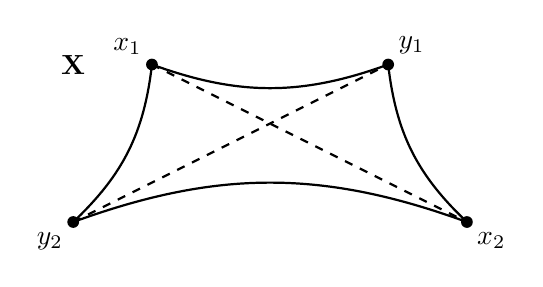
\begin{tikzpicture}
		\draw (0,2) node{$\mathbf{X}$};
		\draw [thick] (0,0) node[anchor=north east]{$y_2$}
			to [bend angle=20, bend right] (1,2) node[anchor=south east]{$x_1$}
			to [bend angle=20, bend right] (4,2) node[anchor=south west]{$y_1$}
			to [bend angle=20, bend right] (5,0) node[anchor=north west]{$x_2$}
			to [bend angle=20, bend right] cycle;
		\draw [thick, dashed] (0,0) -- (4,2);
		\draw [thick, dashed] (1,2) -- (5,0);
		
		\draw (0,0) node[fill,circle,inner sep=1.5pt]{};
		\draw (1,2) node[fill,circle,inner sep=1.5pt]{};
		\draw (5,0) node[fill,circle,inner sep=1.5pt]{};
		\draw (4,2) node[fill,circle,inner sep=1.5pt]{};
	\end{tikzpicture}
	\hspace{1.5cm}
	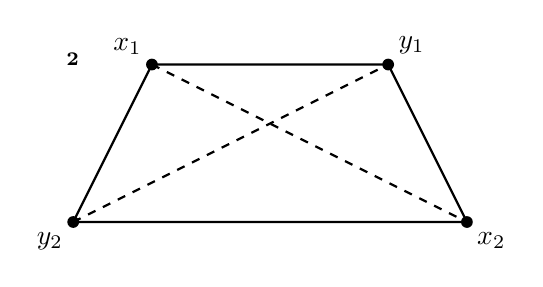
\begin{tikzpicture}
		\draw (0,2) node{$\mathbf{\EE^2}$};
		\draw [thick] (0,0) node[anchor=north east]{$\ol{y_2}$}
		to (1,2) node[anchor=south east]{$\ol{x_1}$}
		to (4,2) node[anchor=south west]{$\ol{y_1}$}
		to (5,0) node[anchor=north west]{$\ol{x_2}$}
		to cycle;
		\draw [thick, dashed] (0,0) -- (4,2);
		\draw [thick, dashed] (1,2) -- (5,0);
		
		\draw (0,0) node[fill,circle,inner sep=1.5pt]{};
		\draw (1,2) node[fill,circle,inner sep=1.5pt]{};
		\draw (5,0) node[fill,circle,inner sep=1.5pt]{};
		\draw (4,2) node[fill,circle,inner sep=1.5pt]{};
	\end{tikzpicture}
\end{figure}
	
Wir werden sehen, dass man $\CAT$-Räume über die Vierpunktbedingung charakterisieren kann.

\begin{lemma}
\label{lemma:1.37}
	Ein geodätischer Raum ist genau dann $\CAT$, wenn für jedes geodätische Dreieck $\Delta(x,y,z,\alpha,\beta,\gamma)$ mit Vergleichsdreieck $\ol{\Delta}(\ol{x},\ol{y},\ol{z},\ol{\alpha},\ol{\beta},\ol{\gamma})$ in $\EE^2$ gilt:
	$d(x,\beta(s)) \leq d_2(\ol{x},\ol{\beta}(s))$ für alle $s \in [0,d(y,z)]$. (\autoref{aufg:3.2})
\end{lemma}

\begin{figure}[h]
	\centering
	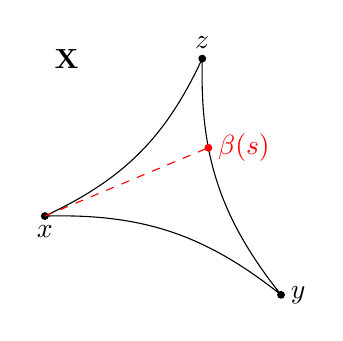
\begin{tikzpicture}[scale=1]
	\draw (0,1) node[fill,circle,inner sep=1pt]{}
	to [bend angle=20, bend left] (3,0) node[fill,circle,inner sep=1pt]{} 
	to [bend angle=20, bend left] coordinate[pos=.66] (M) (2,3) node[fill,circle,inner sep=1pt]{}
	to [bend angle=20, bend left] cycle;
	\draw (0,1) node[below]{$x$};
	\draw (3,0) node[right]{$y$};
	\draw (2,3) node[above]{$z$};
	\draw (M) node[fill,circle,inner sep=1pt,color=red]{};
	\draw (M) node[right,color=red]{$\beta(s)$};
	\draw[color=red, dashed] (0,1) -- (M);
	\draw (0,3) node[right]{$\mathbf{X}$};
	\end{tikzpicture} \hspace{2cm}
	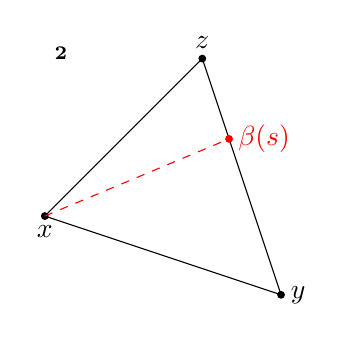
\begin{tikzpicture}[scale=1]
	\draw (0,1) node[fill,circle,inner sep=1pt]{}
	to (3,0) node[fill,circle,inner sep=1pt]{} 
	to coordinate[pos=.66] (M) (2,3) node[fill,circle,inner sep=1pt]{}
	to cycle;
	\draw (0,1) node[below]{$\ol{x}$};
	\draw (3,0) node[right]{$\ol{y}$};
	\draw (2,3) node[above]{$\ol{z}$};
	\draw (M) node[fill,circle,inner sep=1pt,color=red]{};
	\draw (M) node[right,color=red,xshift=-.2]{$\ol{\beta}(s)$};
	\draw[color=red, dashed] (0,1) -- (M);
	\draw (0,3) node[right]{$\mathbf{\EE^2}$};
	\end{tikzpicture}	
\end{figure}

\begin{theorem}
\label{thm:1.38}
	Ein vollständiger metrischer Raum ist $\CAT$ genau dann, wenn er ungefähre Mittelpunkte hat und die $\CAT$-Vierpunktbedingung erfüllt.
\end{theorem}	

\begin{beweis}
	\mbox{} \\[-.8cm]
	\begin{description}
		\item[\bewhin] Der Raum $X$ sei $\CAT$.
		Dann hat $X$ Mittelpunkte, also auch ungefähre Mittelpunkte.
		Seien $x_1,y_1,x_2,y_2 \in X$.
		Betrachte die euklidischen Vergleichsdreiecke zu $\Delta(x_1,x_2,y_2)$ und $\Delta(x_1,x_2,y_2)$. Das resultierende Viereck ist entweder konvex oder nicht.
	\begin{description}
		\item[1. Fall:] Das Viereck ist konvex.
		
		\begin{figure}[h]
			\centering
			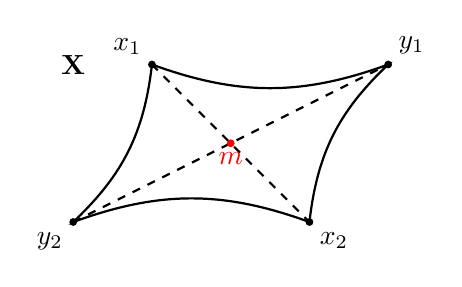
\begin{tikzpicture}
			\draw (0,2) node{$\mathbf{X}$};
			\draw [thick] (0,0) node[anchor=north east]{$y_2$}
			to [bend angle=20, bend left] (3,0) node[anchor=north west]{$x_2$}
			to [bend angle=20, bend left] (4,2) node[anchor=south west]{$y_1$}
			to [bend angle=20, bend left] (1,2) node[anchor=south east]{$x_1$}
			to [bend angle=20, bend left] cycle;
			
			\draw [dashed, thick] (0,0) -- (4,2);
			\draw [dashed, thick] (1,2) -- (3,0);
			
			\draw (0,0) node[fill,circle,inner sep=1pt]{};
			\draw (3,0) node[fill,circle,inner sep=1pt]{};
			\draw (1,2) node[fill,circle,inner sep=1pt]{};
			\draw (4,2) node[fill,circle,inner sep=1pt]{};
			
			\draw (2,1) node[fill,circle,inner sep=1pt,color=red]{};
			\draw (2,1) node[below,color=red]{$m$};
			\end{tikzpicture} \hspace{1.5cm}
			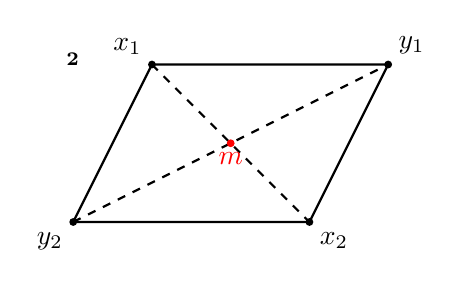
\begin{tikzpicture}
			\draw (0,2) node{$\mathbf{\EE^2}$};
			\draw [thick] (0,0) node[anchor=north east]{$\ol{y_2}$}
			to (3,0) node[anchor=north west]{$\ol{x_2}$}
			to (4,2) node[anchor=south west]{$\ol{y_1}$}
			to (1,2) node[anchor=south east]{$\ol{x_1}$}
			to cycle;
			
			\draw [dashed, thick] (0,0) -- (4,2);
			\draw [dashed, thick] (1,2) -- (3,0);
			
			\draw (0,0) node[fill,circle,inner sep=1pt]{};
			\draw (3,0) node[fill,circle,inner sep=1pt]{};
			\draw (1,2) node[fill,circle,inner sep=1pt]{};
			\draw (4,2) node[fill,circle,inner sep=1pt]{};
			
			\draw (2,1) node[fill,circle,inner sep=1pt,color=red]{};
			\draw (2,1) node[below,color=red]{$\ol{m}$};
			\end{tikzpicture}
		\end{figure} 
		
		Definiere $\ol{m}$ als Schnittpunkt der beiden Diagonalen in $\EE^2$ und sei $t$ so, dass $\ol{\alpha}(t) = \ol{m}$ für $\ol{\alpha}\colon \ol{x_1} \geo \ol{x_2}$. Setze dann $m := \alpha(t)$.
		
		Da $X$ $\CAT$ ist, gilt $d(y_2,m) \leq d_2(\ol{y_2},\ol{m})$ sowie $d(y_1,m) \leq d_2(\ol{y_1},\ol{m})$.
		Da $\ol{m}$ auf der Geodäte zwischen $\ol{y_1}$ und $\ol{y_2}$ liegt, erhalten wir insgesamt:
		\begin{align*}
			d(y_1,y_2) &\stack{\Delta\text{-Ungl.}}{=} d(y_1,m) + d(m,y_2) \\
			&\stack{}{\leq} d_2(\ol{y_1},\ol{m}) + d_2(\ol{m},\ol{y_2}) = d_2(\ol{y_1},\ol{y_2})
		\end{align*}
		\item[2. Fall:] Das Viereck ist nicht konvex.
		
		\begin{figure}[h]
			\centering
			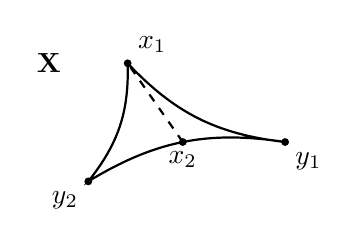
\begin{tikzpicture}
			\draw (0,2) node{$\mathbf{X}$};
			\draw [thick] (0.5,0.5) node[anchor=north east]{$y_2$}
			to [bend angle=20, bend left] coordinate[pos=.5] (X) (3,1) node[anchor=north west]{$y_1$}
			to [bend angle=20, bend left] (1,2) node[anchor=south west]{$x_1$}
			to [bend angle=20, bend left] cycle;
			
			\draw [dashed, thick] (X) -- (1,2);
			\draw (X) node[below]{$x_2$};
			
			
			\draw (0.5,0.5) node[fill,circle,inner sep=1pt]{};
			\draw (X) node[fill,circle,inner sep=1pt]{};
			\draw (1,2) node[fill,circle,inner sep=1pt]{};
			\draw (3,1) node[fill,circle,inner sep=1pt]{};	
			\end{tikzpicture} \hspace{1.5cm}
			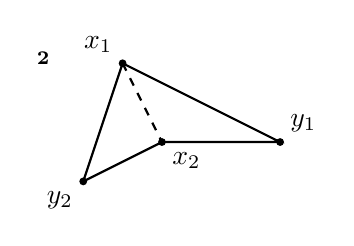
\begin{tikzpicture}
			\draw (0,2) node{$\mathbf{\EE^2}$};
			\draw [thick] (0.5,0.5) node[anchor=north east]{$\ol{y_2}$}
			to (1.5,1) node[anchor=north west]{$\ol{x_2}$}
			to (3,1) node[anchor=south west]{$\ol{y_1}$}
			to (1,2) node[anchor=south east]{$\ol{x_1}$}
			to cycle;
			
			\draw [dashed, thick] (1,2) -- (1.5,1);
			
			\draw (0.5,0.5) node[fill,circle,inner sep=1pt]{};
			\draw (1.5,1) node[fill,circle,inner sep=1pt]{};
			\draw (3,1) node[fill,circle,inner sep=1pt]{};
			\draw (1,2) node[fill,circle,inner sep=1pt]{};
			\end{tikzpicture}
		\end{figure}
		
		Betrachte dann folgendes Dreieck in $\EE^2$ mit
		\[
			\begin{array}{cc}
				d_2(\ol{x_2},\ol{y_2}) = d_2(\ol{\ol{x_2}},\ol{\ol{y_2}}), &
				d_2(\ol{x_2},\ol{y_1}) = d_2(\ol{\ol{x_2}},\ol{\ol{y_1}}), \\
				d_2(\ol{x_1},\ol{y_1}) = d_2(\ol{\ol{x_1}},\ol{\ol{y_1}}), &
				d_2(\ol{x_1},\ol{y_2}) = d_2(\ol{\ol{x_1}},\ol{\ol{y_2}}).			
			\end{array}
		\]
		
		\begin{figure}[h]
			\centering
			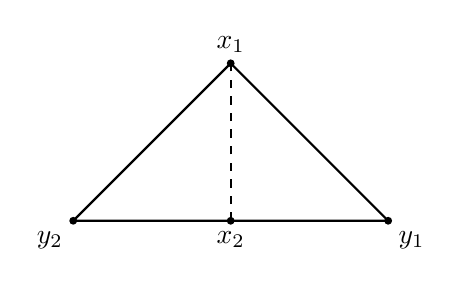
\begin{tikzpicture}
			\draw [thick] (0,0) node[anchor=north east]{$\ol{\ol{y_2}}$}
			to (2,0) node[anchor=north]{$\ol{\ol{x_2}}$}
			to (4,0) node[anchor=north west]{$\ol{\ol{y_1}}$}
			to (2,2) node[anchor=south]{$\ol{\ol{x_1}}$}
			to cycle;
			
			\draw [dashed, thick] (2,0) -- (2,2);
			
			\draw (0,0) node[fill,circle,inner sep=1pt]{};
			\draw (2,0) node[fill,circle,inner sep=1pt]{};
			\draw (4,0) node[fill,circle,inner sep=1pt]{};
			\draw (2,2) node[fill,circle,inner sep=1pt]{};
			\end{tikzpicture}
		\end{figure}
		
		Es gilt
		\[
			d_2(\ol{\ol{x_1}},\ol{\ol{x_2}}) \geq d_2(\ol{x_1},\ol{x_2}) = d_2(x_1,x_2)
		\]
		sowie
		\begin{align*}
			d_2(\ol{\ol{y_1}},\ol{\ol{y_2}}) &\stack{}{=} d_2(\ol{\ol{y_1}},\ol{\ol{x_2}}) + d_2(\ol{\ol{x_2}},\ol{\ol{y_2}}) \\
			&\stack{}{=} d_2(\ol{\ol{y_1}},\ol{\ol{x_2}}) + d_2(\ol{x_2},\ol{y_2}) \\
			&\stack{}{=} d(y_1,x_2) + d(x_2,y_2) \\
			&\stack{\Delta\text{-Ungl.}}{\geq} d(y_1,y_2).
		\end{align*}
	\end{description}
	\item[\bewrueck] Nun sei $X$ vollständig, habe ungefähre Mittelpunkte und erfülle die $\CAT$-Vierpunktbedingung. \marginnote{11.11.15 \\ \ [6]}
	Zuerst zeigen wir, dass $X$ geodätisch ist.
	Nach \autoref{lemma:1.35} reicht es zu zeigen, dass $X$ Mittelpunkte hat.
	Seien $u,v \in X$ beliebig.
	Sei weiter $\varepsilon_n := \frac{1}{n}$ für $n \in \NN$.
	Da $X$ ungefähre Mittelpunkte hat, existiert ein $m_r \in X$ mit $d(u,m_r), d(v,m_r) \leq \frac{1}{2} d(u,v) + \varepsilon_r$.
	Sei $(m_r)_{r \in \NN}$ eine Folge von ungefähren Mittelpunkten mit Fehlerterm $\varepsilon_r := \frac{1}{r}$.
	Unser Ziel ist es zu zeigen, dass $(m_r)_{r}$ eine Cauchy-Folge ist.
	Der Grenzwert $m := \lim_{r \rightarrow \infty} m_r$ ist dann ein Mittelpunkt, denn:
	\begin{align*}
		d(u,m_r) &\leq \frac{1}{2} d(u,v) + \varepsilon_r \\
		\xRightarrow{\lim} \quad \lim\limits_{r \rightarrow \infty} d(u,m_r) &\leq \frac{1}{2} d(u,v) \\
		\xRightarrow{d \text{ stetig}} \quad d(u,m) &\leq \frac{1}{2} d(u,v).
	\end{align*}

	Ebenso erhalten wir $d(v,m) \leq \frac{1}{2} d(u,v)$ und insgesamt $d(u,m) + d(m,v) \leq d(u,v)$. Es gilt aber auch die Dreiecksungleichung $d(u,m) + d(m,v) \geq d(u,v)$. Folglich erhalten wir Gleichheit
	\[
		\Underbrace{d(u,m)}{\leq \frac{1}{2} d(u,v)} + \Underbrace{d(m,v)}{\leq \frac{1}{2} d(u,v)} = d(u,v)
	\]
	und damit $d(u,m) = d(m,v) = \frac{1}{2} d(u,v)$.
	
	Sei nun $\varepsilon > 0$ und $\delta > 0$ die positive Lösung von $-\varepsilon^2 + 4d^2 + 8r\delta = 0$.
	Wir definieren $d(u,v) =: 2r$. 
	Da $(\varepsilon_r)_{r \in \NN}$ eine Nullfolge ist, existiert ein $N \in \NN$, sodass gilt:
	\begin{equation}
		\left. \begin{array}{r}
			d(u,m_r) \\
			d(v,m_r) \\
			d(u,m_s) \\
			d(v,m_s)		
		\end{array} \right\} \leq r+ \delta \quad \forall r,s \geq N \label{eq:1.38.1}
	\end{equation}
	Betrachte das $4$-Tupel $(u,m_r,v,m_s)$ und die Vergleichspunkte $(\ol{u},\ol{m_r},\ol{v},\ol{m_s})$ in $\EE^2$. Sei $\ol{M}$ der Mittelpunkt von $\ol{u}$ und $\ol{v}$.
	\begin{figure}[h]
		\centering
		\begin{tikzpicture}[scale=1.5,>=Latex]
			\draw (0,.8) node{$\mathbf{X}$};
			\draw [thick] (0,0) node[left]{$u$}
			to [bend angle=20, bend left] (2,-1) node[below]{$m_s$}
			to [bend angle=20, bend left] (3,0) node[right]{$v$}
			to [bend angle=20, bend left] (1,1) node[above]{$m_r$}
			to [bend angle=20, bend left] cycle;
			
			\draw (0,0) -- (3,0);
			\draw (2,-1) -- (1,1);
			
			\draw (0,0) node[fill,circle,inner sep=1pt]{};
			\draw (3,0) node[fill,circle,inner sep=1pt]{};
			\draw (1,1) node[fill,circle,inner sep=1pt]{};
			\draw (2,-1) node[fill,circle,inner sep=1pt]{};
		\end{tikzpicture} \hspace{1cm}
		\begin{tikzpicture}[scale=1.5,>=Latex]
			\draw (0,.8) node{$\mathbf{\EE^2}$};
			\draw [thick] (0,0) node[left]{$\ol{u}$}
			to (2,-1) node[below]{$\ol{m_s}$}
			to (3,0) node[right]{$\ol{v}$}
			to (1,1) node[above]{$\ol{m_r}$}
			to cycle;
			
			\draw (0,0) to coordinate[pos=.45] (M) (3,0);
			\draw (2,-1) -- (1,1);
			
			\draw (M) node[below,color=red]{$\ol{M}$};
			
			\draw (0,0) node[fill,circle,inner sep=1pt]{};
			\draw (3,0) node[fill,circle,inner sep=1pt]{};
			\draw (1,1) node[fill,circle,inner sep=1pt]{};
			\draw (2,-1) node[fill,circle,inner sep=1pt]{};
			\draw (M) node[fill,circle,inner sep=1pt,red]{};
		\end{tikzpicture}
	\end{figure}
	Nach Voraussetzung erfüllt $X$ die $\CAT$-Vierpunktbedingung, also gilt
	\begin{equation}
		\left. \begin{array}{rcl}
			d(u,v) & \leq & d_2(\ol{u},\ol{v}) \\
			d(m_r,m_s) & \leq & d_2(\ol{m_r},\ol{m_s})
		\end{array} \right\} \label{eq:1.38.2}
	\end{equation}
	Aus der Parallelogrammgleichung für $\EE^2$ kann man folgern (siehe Beweis zu \autoref{thm:1.22}):
	\begin{equation}
		d_2(\ol{m_r},\ol{M})^2 = \frac{1}{2} d_2 (\ol{u}, \ol{m_r})^2 + \frac{1}{2} d_2 (\ol{m_r},\ol{v})^2 - \frac{1}{4} d_2(\ol{u},\ol{v})^2 \label{eq:1.38.3}
	\end{equation}
	Analoges erhalten wir für $d_2(\ol{m_s},\ol{M})^2$.
	Nun erhalten wir
	\begin{align*}
		d(m_r,m_s) &\stack{\eqref{eq:1.38.2}}{\leq} d_2(\ol{m_r},\ol{m_s}) \\
		&\stack{\Delta-\text{Ungl.}}{\leq} d_2(\ol{m_r},\ol{M}) + d_2(\ol{M},\ol{m_s}) \\
		&\stack{\eqref{eq:1.38.3}}{=} \sqrt{\frac{1}{2} d_2(\ol{u},\ol{m_r})^2 + \frac{1}{2} d_2(\ol{m_r},\ol{v})^2 - \frac{1}{4} d_2(\ol{u},\ol{v})^2}
		+ \sqrt{\frac{1}{2} d_2(\ol{u},\ol{m_s})^2 + \frac{1}{2} d_2(\ol{m_s},\ol{v})^2 - \frac{1}{4} d_2(\ol{u},\ol{v})^2} \\
		&\stack{}{=} \sqrt{\frac{1}{2} d(u,m_r)^2 + \frac{1}{2} d(m_r,v)^2 - \frac{1}{4} d_2(\ol{u},\ol{v})^2}
		+ \sqrt{\frac{1}{2} d(u,m_s)^2 + \frac{1}{2} d(m_s,v)^2 - \frac{1}{4} d_2(\ol{u},\ol{v})^2} \\
		&\stack{\eqref{eq:1.38.1}}{\leq} 2 \cdot \sqrt{(r+\delta)^2 - \frac{1}{4} d_2(\ol{u},\ol{v})^2} \qquad \forall r,s \geq N \\
		&\stack{\eqref{eq:1.38.2}}{\leq} 2 \cdot \sqrt{(r+\delta)^2 - \frac{1}{4} d(u,v)^2} \qquad \forall r,s \geq N \\
		&\stack{}{=} 2 \cdot \sqrt{r^2 + 2r \delta + \delta^2 - r^2} = \varepsilon \qquad \forall r,s \geq N
	\end{align*}
	Somit ist $(m_r)_r$ eine Cauchy-Folge.
	
	Sei $\Delta(x,y,z,\alpha,\beta,\gamma)$ ein geodätisches Dreieck in $X$.
	Wir betrachten die Bedingung aus \autoref{lemma:1.37}. Sei $p := \beta(s) \in \im(\beta \colon y \geo z)$ beliebig.
	\begin{figure}[h]
		\centering
		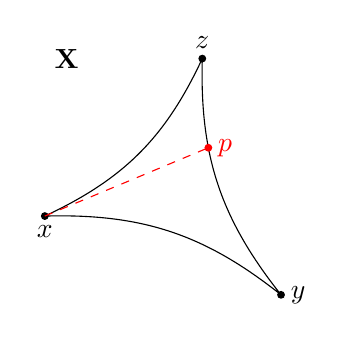
\begin{tikzpicture}[scale=1]
		\draw (0,1) node[fill,circle,inner sep=1pt]{}
		to [bend angle=20, bend left] (3,0) node[fill,circle,inner sep=1pt]{} 
		to [bend angle=20, bend left] coordinate[pos=.66] (M) (2,3) node[fill,circle,inner sep=1pt]{}
		to [bend angle=20, bend left] cycle;
		\draw (0,1) node[below]{$x$};
		\draw (3,0) node[right]{$y$};
		\draw (2,3) node[above]{$z$};
		\draw (M) node[fill,circle,inner sep=1pt,color=red]{};
		\draw (M) node[right,color=red]{$p$};
		\draw[color=red, dashed] (0,1) -- (M);
		\draw (0,3) node[right]{$\mathbf{X}$};
		\end{tikzpicture} \hspace{2cm}
		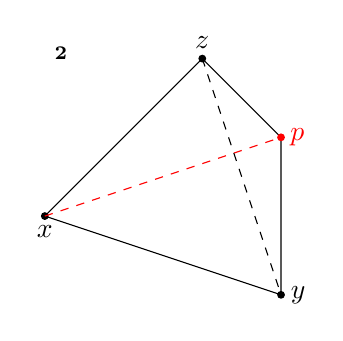
\begin{tikzpicture}[scale=1]
		\draw (0,1) node[fill,circle,inner sep=1pt]{}
		to (3,0) node[fill,circle,inner sep=1pt]{} 
		to (3,2) node[fill,circle,inner sep=1pt,color=red]{} 
		to (2,3) node[fill,circle,inner sep=1pt]{}
		to cycle;
		\draw (0,1) node[below]{$\ol{x}$};
		\draw (3,0) node[right]{$\ol{y}$};
		\draw (2,3) node[above]{$\ol{z}$};
		\draw (3,2) node[right,color=red,xshift=-.2]{$\ol{p}$};
		\draw[color=red, dashed] (0,1) -- (3,2);
		\draw (0,3) node[right]{$\mathbf{\EE^2}$};
		\draw [dashed] (2,3) -- (3,0);
		\end{tikzpicture}	
	\end{figure}
	Zu den Punkten $(x,y,p,z)$ betrachten wir die Vergleichspunkte $(\ol{x},\ol{y},\ol{p},\ol{z})$. Es gilt
	\begin{equation}
		d(x,p) \leq d_2(\ol{x},\ol{p}) \quad \text{und} \quad d(z,y) \leq d_2(\ol{z},\ol{y}) \label{eq:1.38.4}
	\end{equation}
	Wir zeigen, dass $(\ol{x},\ol{y},\ol{p},\ol{z})$ ein Vergleichsdreieck ist, also dass $\ol{p}$ auf der Geodäte $\ol{\beta}\colon \ol{y} \geo \ol{z}$ liegt. Es gilt
	\[
		d_2(\ol{y},\ol{z}) \stack{\eqref{eq:1.38.4}}{\geq} d(y,z) = d(y,p) + d(p,z) = d_2(\ol{y},\ol{p}) + d_2(\ol{p},\ol{z})
	\]
	und
	\[
		d_2(\ol{y},\ol{z} \stack{\Delta-\text{Ungl.}}{\leq} d_2(\ol{y},\ol{p}) + d_2(\ol{p},\ol{z}).
	\]
	Folglich liegt $\ol{p}$ auf der Geodäte $\ol{\beta}$, das heißt wir haben ein Vergleichsdreieck. \qedhere
	\end{description}
\end{beweis}

\begin{theorem}
\label{thm:1.39}
	Die metrische Vervollständigung eines $\CAT$-Raumes ist ein $\CAT$-Raum.
\end{theorem}

\begin{beweis}
	Sei $X$ ein $\CAT$-Raum mit Vervollständigung $\widehat{X}$.
	Wir zeigen, dass die Bedingung aus \autoref{thm:1.38} erfüllt sind.
	Zuerst zeugen wir, dass $\widehat{X}$ ungefähre Mittelpunkte hat.
	Seien $p,q \in \widehat{X}, \varepsilon >0$. Wähle $p',q' \in X$ mit
	\begin{equation}
		d(p,p') < \frac{\varepsilon}{2} \quad \text{und} \quad d(q,q') < \frac{\varepsilon}{2} \label{eq:1.39.1}
	\end{equation}
	und $m' \in X$ als Mittelpunkt von $p'$ und $q'$. Sei $r = d(p,q)$ und $r' = d(p',q')$.
	
	\begin{figure}[h]
		\centering
		\begin{tikzpicture}[scale=1.5,>=Latex]
			\draw [<->,thick] (0,2) node[left]{$p$} -- (4,2) node[right]{$q$};
			\draw [<->,thick] (0.5,0) node[anchor=north east]{$p'$} -- (2,0) node[anchor=north]{$m'$};
			\draw [<->,thick] (2,0) -- (3.5,0) node[anchor=north west]{$q'$};
			\draw [<->,thick] (0.5,0) -- (0,2);
			\draw [<->,thick] (3.5,0) -- (4,2);
			
			\draw (0.5,0) node[fill,circle,inner sep=2pt]{};
			\draw (2,0) node[fill,circle,inner sep=2pt]{};
			\draw (3.5,0) node[fill,circle,inner sep=2pt]{};
			\draw (0,2) node[fill,circle,inner sep=2pt]{};
			\draw (4,2) node[fill,circle,inner sep=2pt]{};
			
			\draw (1.25,0) node[above]{$\dfrac{r'}{2}$};
			\draw (2.75,0) node[above]{$\dfrac{r'}{2}$};
			\draw (0.25,1) node[right]{$\dfrac{\varepsilon}{2}$};
			\draw (3.75,1) node[left]{$\dfrac{\varepsilon}{2}$};
			\draw (2,2) node[below]{$r$};
		\end{tikzpicture}
	\end{figure}
	
	Wir erhalten mit $r' = d(p',q') \leq d(p',p) + d(p,q) + d(q,q') \leq \varepsilon + r$:
	\begin{align*}
		d(p,m') &\stack{\Delta\text{-Ungl.}}{\leq} d(p,p') + d(p',m') \\
		&\stack{\eqref{eq:1.39.1}}{\leq} \frac{\varepsilon}{2} + \frac{r'}{2} \\
		&\stack{}{\leq} \frac{\varepsilon}{2} + \frac{\varepsilon}{2} + \frac{r}{2} = \frac{r}{2} + \varepsilon.
	\end{align*}
	
	und ebenso $d(q,m') \leq \frac{r}{2} + \varepsilon$, das heißt $\widehat{X}$ hat ungefähre Mittelpunkte.
	
	Sei jetzt $(x_1,y_1,x_2,y_2) \in \widehat{X}^4$. Wähle Folgen in $X$ mit
	\[
		x_1(n) \rightarrow x_1 \qquad y_1(n) \rightarrow y_1 \qquad x_2(n) \rightarrow x_2 \qquad y_2(n) \rightarrow y_2
	\]
	und $\CAT$-Vierpunkt-Vergleichspunkte $\ol{x_1(n)}, \ol{y_1(n)}, \ol{x_2(n)}, \ol{y_2(n)}$ in $\EE^2$. Ohne Einschränkung sei $\ol{x_1(n)} = 0$ für alle $n \in \NN$. Die Folge $(\ol{x_1(n)}, \ol{y_1(n)}, \ol{x_2(n)}, \ol{y_2(n)})$ hat einen Häufungspunkt in $(\EE^2)^4$, weil sie beschränkt ist. Wir dürfen ohne Einschränkung annehmen, dass wir Konvergenz haben, das heißt
	\[
		\lim\limits_{n \rightarrow \infty} (\ol{x_1(n)}, \ol{y_1(n)}, \ol{x_2(n)}, \ol{y_2(n)}) = (0,\ol{y_1},\ol{x_1},\ol{x_2}).
	\]
	Dann folgt:
	\begin{align*}
		d(x_i,y_j) &\stack{}{=} d\enbrace*{\lim\limits_{n} x_i(n), \lim\limits_n y_j(n)} \\
		&\stack{d\text{ stetig}}{=} \lim\limits_{n} d(x_i(n),y_j(n)) \\
		&\stack{}{=} \lim\limits_{n} d_2(\ol{x_i(n)},\ol{y_j(n)}) \\
		&\stack{d_2\text{ stetig}}{=} d_2(\ol{x_i},\ol{y_j})
	\end{align*}
	Ebenso haben wir $d(x_1,x_2) \leq d_2(\ol{x_1},\ol{x_2})$ und $d(y_1,y_2) \leq d_2(\ol{y_1},\ol{y_2})$. \qedhere
\end{beweis}
\cleardoubleoddemptypage